% !TeX program = xelatex
% !TeX encoding = UTF-8
% Spedizione P03 · Il Nilo: livelli e dipendenza temporale
% Presentazione della spedizione P03 nella serie planetaria di GeoStat Lab.
% Compilazione: xelatex -interaction=nonstopmode P03_Nilo.tex (due passaggi)
% 31 slide. Diagrammi TikZ, figure vettoriali da R/P03_figure.R, codice R, dati ed esperimenti inclusi.
\RequirePackage{fix-cm}
\documentclass[12pt,aspectratio=1610]{beamer}
\geometry{paperwidth=20cm,paperheight=12.5cm}
\usepackage[italian,provide=*]{babel}
\usepackage{fontspec,adjustbox,tabularx}
\IfFontExistsTF{NimbusSans-Regular.otf}{
\setsansfont{NimbusSans-Regular.otf}[BoldFont=NimbusSans-Bold.otf,ItalicFont=NimbusSans-Italic.otf,BoldItalicFont=NimbusSans-BoldItalic.otf]
\setmainfont{NimbusSans-Regular.otf}[BoldFont=NimbusSans-Bold.otf,ItalicFont=NimbusSans-Italic.otf,BoldItalicFont=NimbusSans-BoldItalic.otf]
}{
\setsansfont{TeX Gyre Heros}
\setmainfont{TeX Gyre Heros}
}
\IfFontExistsTF{DejaVu Sans Mono}{
\setmonofont{DejaVu Sans Mono}[Scale=.88]
}{\setmonofont{Latin Modern Mono}[Scale=.88]}
\usefonttheme{professionalfonts}
\usepackage{amsmath,amssymb,booktabs,array,graphicx,tikz,bookmark}
\usetikzlibrary{calc,positioning,arrows.meta}
\graphicspath{{Figure/}}
\definecolor{Paper}{HTML}{F8F6F1}
\definecolor{Ink}{HTML}{253344}
\definecolor{Navy}{HTML}{15283E}
\definecolor{Quantum}{HTML}{5146A5}
\definecolor{Classical}{HTML}{087C74}
\definecolor{Muted}{HTML}{657180}
\definecolor{Rule}{HTML}{D6DAD9}
\definecolor{Night}{HTML}{112236}
\definecolor{Lilac}{HTML}{ABB5FF}
\definecolor{Mint}{HTML}{72D8C8}
\setbeamercolor{background canvas}{bg=Paper}
\setbeamercolor{normal text}{fg=Ink}
\setbeamertemplate{navigation symbols}{}
\setbeamertemplate{headline}{}
\setbeamertemplate{footline}{}
\setbeamersize{text margin left=0pt,text margin right=0pt}
\hypersetup{colorlinks=true,linkcolor=Classical,urlcolor=Classical,pdfpagemode=UseOutlines,pdfstartview=Fit,
 pdftitle={Spedizione P03 · Il Nilo: livelli e dipendenza temporale},pdfauthor={GeoStat Lab · materiali di Marzio De Corato},
 pdfsubject={GeoStat Lab · P03}}
\bookmarksetup{open,openlevel=0,depth=2}
\newsavebox{\BodyBox}
\newsavebox{\SideBox}
\newsavebox{\RecallBox}
\newsavebox{\TitleBox}
\newcommand{\MeasureBox}[2]{\typeout{REVIEWBOX:#1:\the\wd#2:\the\ht#2:\the\dp#2}}

% Revisione completa: diagrammi TikZ, formalismo e box R.
\usepackage[most]{tcolorbox}
\usepackage{listings}
\usetikzlibrary{fit,backgrounds,matrix,decorations.pathreplacing}
\definecolor{GeoA}{HTML}{1D7890}
\definecolor{GeoB}{HTML}{C57E42}
\definecolor{GeoC}{HTML}{7363AA}
\definecolor{GeoTint}{HTML}{F0F4F3}
\lstdefinestyle{GeoR}{language=R,basicstyle=\ttfamily\fontsize{9.2}{12.2}\selectfont,
 keywordstyle=\color{Quantum}\bfseries,commentstyle=\color{Classical},stringstyle=\color{GeoB},
 numbers=left,numberstyle=\tiny\color{Muted},numbersep=4pt,showstringspaces=false,
 columns=fullflexible,keepspaces=true,breaklines=true,xleftmargin=1.15em,
 frame=none,aboveskip=0pt,belowskip=0pt,tabsize=2}
\newsavebox{\PilotLeftBox}
\newsavebox{\PilotRightBox}
\newcommand{\PLabel}[1]{\par{\color{Classical}\bfseries\fontsize{9}{11}\selectfont\MakeUppercase{#1}}\par\vspace{1.8mm}}
\newcommand{\PBody}[1]{\par{\fontsize{11.3}{14.8}\selectfont #1\par}}
\newcommand{\PSmall}[1]{\par{\fontsize{9.8}{13.1}\selectfont #1\par}}
\newcommand{\PCode}[2]{%
\begin{tcolorbox}[enhanced,arc=1.8mm,boxrule=.65pt,
  colback=white,colframe=Classical!75!Navy,colbacktitle=Navy,
  coltitle=white,fonttitle=\bfseries\fontsize{9.6}{12}\selectfont,
  title={#1},left=1.7mm,right=1.3mm,top=1.5mm,bottom=1.3mm,
  before skip=1mm,after skip=1mm]
\lstinputlisting[style=GeoR]{Codice/#2}
\end{tcolorbox}}
\newcommand{\PInfo}[1]{%
\begin{tcolorbox}[enhanced,arc=1.6mm,boxrule=.55pt,colback=GeoTint,
 colframe=Rule!80!Classical,left=2.3mm,right=2.3mm,top=2mm,bottom=2mm,
 before skip=1mm,after skip=1mm]
\PSmall{#1}\end{tcolorbox}}
\tikzset{
 pFlow/.style={draw=Classical!45,fill=white,rounded corners=2mm,
  line width=.7pt,align=center,minimum height=1.1cm,font=\sffamily\fontsize{10}{12}\selectfont},
 pEdge/.style={-{Latex[length=2.3mm]},draw=Classical,line width=.95pt},
 pGroup/.style={draw=Rule,fill=white,rounded corners=2mm,line width=.65pt},
 pDotA/.style={circle,fill=GeoA,inner sep=1.25pt},
 pDotB/.style={circle,fill=GeoB,inner sep=1.25pt},
 pDotC/.style={circle,fill=GeoC,inner sep=1.25pt}
}
\newcommand{\PilotChrome}[4]{%
  \node[anchor=north west,inner sep=0,text width=17.7cm] at ([xshift=.95cm,yshift=-.55cm]current page.north west) {\color{Navy}\bfseries\fontsize{20.6}{24.5}\selectfont #1};
  \node[anchor=north east,inner sep=0] at ([xshift=19.05cm,yshift=-.14cm]current page.north west) {\color{Classical}\fontsize{8}{10}\selectfont\hyperlink{slide2}{#2}};
  \draw[Classical,line width=1.2pt] ([xshift=.95cm,yshift=-1.7cm]current page.north west)--([xshift=2.35cm,yshift=-1.7cm]current page.north west);
  \draw[Rule,line width=.65pt] ([xshift=.95cm,yshift=-10.36cm]current page.north west)--([xshift=19.05cm,yshift=-10.36cm]current page.north west);
  \node[anchor=north west,inner sep=0] at ([xshift=.96cm,yshift=-10.55cm]current page.north west) {\color{Classical}\bfseries\fontsize{9.1}{12}\selectfont DA RICORDARE};
  \node[anchor=north west,inner sep=0,text width=14.3cm] at ([xshift=4.2cm,yshift=-10.53cm]current page.north west) {\color{Ink}\fontsize{10.3}{13.8}\selectfont #4};
  \draw[Rule,line width=.35pt] ([xshift=.95cm,yshift=-11.92cm]current page.north west)--([xshift=19.05cm,yshift=-11.92cm]current page.north west);
  \node[anchor=north west,inner sep=0] at ([xshift=.95cm,yshift=-12.06cm]current page.north west) {\color{Muted}\fontsize{7.7}{9.2}\selectfont Spedizione P03 · Il Nilo: livelli e dipendenza temporale};
  \node[anchor=north east,inner sep=0] at ([xshift=19.05cm,yshift=-12.06cm]current page.north west) {\color{Muted}\fontsize{7.7}{9.2}\selectfont #3/31};
}


% Stili comuni per i diagrammi scientifici della revisione completa.
\tikzset{
 pAxis/.style={-{Latex[length=2mm]},draw=Muted,line width=.65pt},
 pNote/.style={font=\sffamily\fontsize{9}{11.5}\selectfont,text=Muted,align=center},
 pLabel/.style={font=\sffamily\fontsize{10}{12.5}\selectfont,text=Ink,align=center}
}
\newsavebox{\FullWideBox}
\setlength{\emergencystretch}{1em}




\newcommand{\PLab}[2]{\par{\color{Classical}\bfseries\fontsize{9}{11}\selectfont
\href{#1}{\MakeUppercase{#2}}}\par\vspace{1.8mm}}

\definecolor{Measure}{HTML}{A05B10}\definecolor{Rose}{HTML}{9B4564}\definecolor{Wash}{HTML}{EAE7F6}\definecolor{Gold}{HTML}{EEC184}
\tikzset{arr/.style={-{Stealth[length=2mm]},line width=.8pt,draw=Classical}}
\newcommand{\Colonna}[2]{\begin{adjustbox}{max totalsize={#1}{7.95cm},valign=t}\begin{minipage}[t]{#1}\raggedright\fontsize{11.3}{14.8}\selectfont #2\end{minipage}\end{adjustbox}}
\begin{document}

\begin{frame}[plain]\hypertarget{slide1}{}\bookmark[level=0,page=1]{Spedizione P03}
\begin{tikzpicture}[remember picture,overlay]
\fill[Night](current page.south west) rectangle(current page.north east);
\IfFileExists{Scena/copertina.jpg}{\node[inner sep=0] at(current page.center){
\includegraphics[width=20cm,height=12.5cm]{Scena/copertina.jpg}};}{}
\node[anchor=north west,inner sep=0] at([xshift=1.05cm,yshift=-1.10cm]current page.north west){\color{Mint}\bfseries\fontsize{23}{28}\selectfont SPEDIZIONE P03};
\node[anchor=north west,inner sep=0] at([xshift=1.07cm,yshift=-2.16cm]current page.north west){\color{white}\fontsize{9}{12}\selectfont MACROPROGETTO P03 · SCIENZE DELLA TERRA};
\draw[Mint,line width=1.5pt]([xshift=1.07cm,yshift=-2.78cm]current page.north west)--([xshift=2.6cm,yshift=-2.78cm]current page.north west);
\node[anchor=north west,inner sep=0] at([xshift=1.05cm,yshift=-3.35cm]current page.north west){\begin{minipage}{9.2cm}\raggedright\color{white}\bfseries\fontsize{28.5}{34.5}\selectfont Il Nilo: livelli\\e dipendenza\\temporale\end{minipage}};
\node[anchor=north west,inner sep=0] at([xshift=1.07cm,yshift=-7.88cm]current page.north west){\begin{minipage}{8.9cm}\raggedright\color{Lilac}\fontsize{12.2}{17}\selectfont Cento anni di volumi ad Aswan\end{minipage}};
\node[anchor=north west,inner sep=0] at([xshift=1.07cm,yshift=-8.70cm]current page.north west){\begin{minipage}{8.9cm}\raggedright\color{white!75}\fontsize{10.3}{14.5}\selectfont Volumi annuali, contrasto fra periodi e covarianza HAC\end{minipage}};
\node[anchor=north west,inner sep=0] at([xshift=1.07cm,yshift=-10.52cm]current page.north west){\color{white}\fontsize{10.5}{14}\selectfont GeoStat Lab · corso di Marzio De Corato};
\node[anchor=north west,inner sep=0] at([xshift=1.07cm,yshift=-11.17cm]current page.north west){\color{Mint}\fontsize{8.8}{11}\selectfont\href{https://creativecommons.org/licenses/by-nc-sa/4.0/}{Impaginazione da Tessera · CC BY-NC-SA 4.0}};
\end{tikzpicture}\end{frame}

\begin{frame}[plain]\hypertarget{slide2}{}
\bookmark[level=1,page=2]{Indice della presentazione}
\begin{tikzpicture}[remember picture,overlay]
\PilotChrome{Indice della presentazione}{PERCORSO}{2}{I titoli dell’indice aprono i capitoli. Il nome del capitolo in alto riporta a questa pagina.}
\node[anchor=north west,inner sep=0] at([xshift=.96cm,yshift=-2.12cm]current page.north west){\Colonna{9.40cm}{\PLabel{Capitoli}
{\fontsize{10.7}{13.5}\selectfont\hyperlink{slide4}{Serie storica e contrasto dichiarato\hfill 4}\par}\vspace{.16cm}
{\fontsize{10.7}{13.5}\selectfont\hyperlink{slide9}{Modello del livello e residui\hfill 9}\par}\vspace{.16cm}
{\fontsize{10.7}{13.5}\selectfont\hyperlink{slide14}{Covarianza HAC e analisi di sensibilità\hfill 14}\par}\vspace{.16cm}
{\fontsize{10.7}{13.5}\selectfont\hyperlink{slide21}{Interpretazione idrologica e consegna\hfill 21}\par}\vspace{.16cm}
{\fontsize{10.7}{13.5}\selectfont\hyperlink{slide23}{Laboratori della spedizione\hfill 23}\par}\vspace{.16cm}

}};
\node[anchor=north west,inner sep=0] at([xshift=10.85cm,yshift=-2.12cm]current page.north west){\Colonna{8.16cm}{\PLabel{Percorso di lettura}
\PBody{Il percorso controlla la serie e il contrasto dichiarato, stima la differenza con un modello del livello, esamina i residui e ricalcola l’incertezza con la covarianza HAC. I laboratori finali riprendono le tre fasi della spedizione.}
\PInfo{Le pagine Scenario A e Confronto riprendono gli esperimenti nel browser con dati sintetici. I valori di partenza del simulatore differiscono da quelli del caso.}
\href{https://marzione00.github.io/Lab_Geo/\#modulo-P03}{\color{Classical}\bfseries Apri la spedizione P03 su GeoStat Lab}
}};
\end{tikzpicture}\end{frame}

\begin{frame}[plain]\hypertarget{slide3}{}
\bookmark[level=1,page=3]{Di quanto diminuisce il volume annuale del Nilo dopo il 1898, e quanto pesa la dipendenza fra anni?}
\begin{tikzpicture}[remember picture,overlay]
\PilotChrome{{\fontsize{15.3}{19}\selectfont Di quanto diminuisce il volume annuale del Nilo dopo il 1898, e quanto pesa la dipendenza fra anni?}}{IL CASO GUIDA}{3}{La copertina è una scena illustrativa: le colonne riproducono i cento volumi della serie Nile.}
\node[anchor=north west,inner sep=0] at([xshift=.96cm,yshift=-2.12cm]current page.north west){\Colonna{9.40cm}{{\centering\resizebox{0.97\linewidth}{!}{\begin{tikzpicture}[x=1cm,y=1cm,every node/.style={font=\sffamily\fontsize{10}{12}\selectfont,text=Ink}]
\draw[draw=Classical,fill=Classical!8,rounded corners=2mm,line width=.7pt] (0,0.00) rectangle (8.6,-0.78);
\node[circle,anchor=center,fill=Classical,inner sep=0,minimum size=.5cm,text=white,font=\sffamily\bfseries\fontsize{9}{10}\selectfont] at (.48,-0.39) {1};
\node[anchor=west,text width=7.4cm,align=left] at (.95,-0.39) {Serie storica e contrasto dichiarato};
\draw[pEdge] (.48,-0.80)--(.48,-1.02);
\draw[draw=Classical,fill=Classical!8,rounded corners=2mm,line width=.7pt] (0,-1.04) rectangle (8.6,-1.82);
\node[circle,anchor=center,fill=Classical,inner sep=0,minimum size=.5cm,text=white,font=\sffamily\bfseries\fontsize{9}{10}\selectfont] at (.48,-1.43) {2};
\node[anchor=west,text width=7.4cm,align=left] at (.95,-1.43) {Modello del livello e residui};
\draw[pEdge] (.48,-1.84)--(.48,-2.06);
\draw[draw=Classical,fill=Classical!8,rounded corners=2mm,line width=.7pt] (0,-2.08) rectangle (8.6,-2.86);
\node[circle,anchor=center,fill=Classical,inner sep=0,minimum size=.5cm,text=white,font=\sffamily\bfseries\fontsize{9}{10}\selectfont] at (.48,-2.47) {3};
\node[anchor=west,text width=7.4cm,align=left] at (.95,-2.47) {Covarianza HAC e analisi di sensibilità};
\draw[pEdge] (.48,-2.88)--(.48,-3.10);
\draw[draw=Classical,fill=Classical!8,rounded corners=2mm,line width=.7pt] (0,-3.12) rectangle (8.6,-3.90);
\node[circle,anchor=center,fill=Classical,inner sep=0,minimum size=.5cm,text=white,font=\sffamily\bfseries\fontsize{9}{10}\selectfont] at (.48,-3.51) {4};
\node[anchor=west,text width=7.4cm,align=left] at (.95,-3.51) {Interpretazione idrologica e consegna};
\draw[pEdge] (.48,-3.92)--(.48,-4.14);
\draw[draw=GeoB,fill=GeoB!8,rounded corners=2mm,line width=.7pt] (0,-4.16) rectangle (8.6,-4.94);
\node[circle,anchor=center,fill=GeoB,inner sep=0,minimum size=.5cm,text=white,font=\sffamily\bfseries\fontsize{9}{10}\selectfont] at (.48,-4.55) {L};
\node[anchor=west,text width=7.4cm,align=left] at (.95,-4.55) {Laboratori della spedizione};
\end{tikzpicture}
}\par}
\PSmall{Capitoli della spedizione; L indica i laboratori conclusivi.}
}};
\node[anchor=north west,inner sep=0] at([xshift=10.85cm,yshift=-2.12cm]current page.north west){\Colonna{8.16cm}{\PLabel{Il caso}
\PBody{La serie Nile di R riporta cento volumi annuali del Nilo ad Aswan, dal 1871 al 1970, in centinaia di milioni di metri cubi. La documentazione segnala un cambiamento vicino al 1898, che la spedizione assume come separazione dichiarata.}
\PInfo{Seguiremo la stessa differenza fra periodi dall’intervallo classico alla covarianza HAC, con la sensibilità al ritardo massimo e alla posizione della soglia.}
}};
\end{tikzpicture}\end{frame}

\begin{frame}[plain]\hypertarget{slide4}{}
\bookmark[level=0,page=4]{Serie storica e contrasto dichiarato}
\bookmark[level=1,page=4]{Una differenza nella serie storica di Aswan}
\begin{tikzpicture}[remember picture,overlay]
\PilotChrome{Una differenza nella serie storica di Aswan}{SERIE STORICA E CONTRASTO DICHIARATO}{4}{L’origine della soglia appartiene al protocollo dell’analisi e ne delimita la forza inferenziale.}
\node[anchor=north west,inner sep=0] at([xshift=.96cm,yshift=-2.12cm]current page.north west){\Colonna{9.40cm}{{\centering\resizebox{0.90\linewidth}{!}{\begin{tikzpicture}[x=1cm,y=-.87cm,every node/.style={font=\fontsize{12.2}{15}\selectfont,text=Ink},arr/.style={-{Stealth[length=2mm]},line width=.8pt,draw=Classical}]\path[use as bounding box] (0,0) rectangle (7.45,6.2);
\draw[Rule,line width=.8pt] (0.5,2.5)--(6.9,2.5);
\draw[Quantum,line width=.8pt] (2.7,1.4)--(2.7,3.5);
\node[anchor=center,text=Ink,font=\fontsize{13}{15}\selectfont,text width=2cm,align=center] at (1.45,1.5) {27 anni};
\node[anchor=center,text=Ink,font=\fontsize{13}{15}\selectfont,text width=3cm,align=center] at (4.8,1.5) {73 anni};
\node[anchor=center,text=Ink,font=\fontsize{11.5}{15}\selectfont,text width=2.5cm,align=center] at (1.45,3.5) {1871–1897};
\node[anchor=center,text=Ink,font=\fontsize{11.5}{15}\selectfont,text width=3cm,align=center] at (4.8,3.5) {1898–1970};
\node[anchor=center,text=Ink,font=\fontsize{12.2}{15}\selectfont,text width=6.7cm,align=center] at (3.7,5.3) {Separazione ripresa dalla documentazione storica};

\end{tikzpicture}}\par}
}};
\node[anchor=north west,inner sep=0] at([xshift=10.85cm,yshift=-2.12cm]current page.north west){\Colonna{8.16cm}{\PBody{Il progetto confronta i volumi annuali del Nilo ad Aswan nei periodi 1871–1897 e 1898–1970, utilizzando la serie Nile distribuita con R. La documentazione segnala già un cambiamento prossimo al 1898, che viene quindi assunto come riferimento di una rianalisi. L’argomento riguarda la grandezza del contrasto e la sensibilità della sua incertezza alla dipendenza temporale. La posizione della soglia, essendo nota attraverso la stessa storia della serie, richiede cautela nel descrivere l’analisi come verifica indipendente di un cambiamento.}
}};
\end{tikzpicture}\end{frame}

\begin{frame}[plain]\hypertarget{slide5}{}
\bookmark[level=1,page=5]{Il volume annuale conserva il proprio denominatore}
\begin{tikzpicture}[remember picture,overlay]
\PilotChrome{Il volume annuale conserva il proprio denominatore}{SERIE STORICA E CONTRASTO DICHIARATO}{5}{La scala temporale della misura deve comparire nell’unità e nella conclusione.}
\node[anchor=north west,inner sep=0] at([xshift=.96cm,yshift=-2.12cm]current page.north west){\Colonna{9.40cm}{{\centering\resizebox{0.90\linewidth}{!}{\begin{tikzpicture}[x=1cm,y=-.87cm,every node/.style={font=\fontsize{12.2}{15}\selectfont,text=Ink},arr/.style={-{Stealth[length=2mm]},line width=.8pt,draw=Classical}]\path[use as bounding box] (0,0) rectangle (7.45,6.2);
\draw[draw=Classical,fill=Classical!8,rounded corners=2pt,line width=.7pt] (0.5,0.6) rectangle (6.9,2);
\node[anchor=center,text=Ink,font=\fontsize{12.2}{15}\selectfont,text width=6cm,align=center] at (3.7,1.3) {Volume integrato in un anno};
\draw[arr,draw=Classical] (3.7,2.2)--(3.7,3.1);
\node[anchor=center,text=Ink,font=\fontsize{11.5}{15}\selectfont,text width=2.6cm,align=center] at (5.2,2.65) {÷ secondi};
\draw[draw=Quantum,fill=Quantum!8,rounded corners=2pt,line width=.7pt] (0.5,3.3) rectangle (6.9,4.7);
\node[anchor=center,text=Ink,font=\fontsize{12.2}{15}\selectfont,text width=6cm,align=center] at (3.7,4) {Portata media dello stesso anno};
\node[anchor=center,text=Ink,font=\fontsize{11}{15}\selectfont,text width=6.7cm,align=center] at (3.7,5.6) {La conversione cambia la scala, non recupera la dinamica interna.};

\end{tikzpicture}}\par}
\PSmall{$y_t$: valore numerico della tabella nell’anno t; $V_t$: volume; $\Delta t_t$: durata dell’anno in secondi; $\bar Q_t$: portata media.}
}};
\node[anchor=north west,inner sep=0] at([xshift=10.85cm,yshift=-2.12cm]current page.north west){\Colonna{8.16cm}{\PBody{Ogni valore misura un volume accumulato nell’anno, espresso in centinaia di milioni di metri cubi. La portata media si otterrebbe dividendo quel volume per la durata effettiva dell’anno in secondi, mentre una portata istantanea richiederebbe una risoluzione osservativa differente. Questa distinzione determina unità e interpretazione della differenza fra periodi. Un valore numerico può apparire plausibile anche quando viene associato all’unità sbagliata, per cui il controllo del dizionario precede la scelta del modello.}
\par\smallskip{\centering\adjustbox{max width=.98\linewidth}{$\displaystyle \begin{gathered}V_t=10^8y_t\ \mathrm{m^3}\\\bar Q_t=V_t/\Delta t_t,\qquad[\bar Q_t]=\mathrm{m^3\,s^{-1}}\end{gathered}$}\par\smallskip}
}};
\end{tikzpicture}\end{frame}

\begin{frame}[plain]\hypertarget{slide6}{}
\bookmark[level=1,page=6]{Controllare la continuità degli anni}
\begin{tikzpicture}[remember picture,overlay]
\PilotChrome{Controllare la continuità degli anni}{SERIE STORICA E CONTRASTO DICHIARATO}{6}{L’ordine temporale e la composizione dei periodi vengono verificati sul dato importato.}
\node[anchor=north west,inner sep=0] at([xshift=.96cm,yshift=-2.12cm]current page.north west){\Colonna{9.40cm}{\PBody{La tabella contiene cento anni consecutivi e viene confrontata numericamente con il dataset originale di R. Il controllo di unicità e ordinamento distingue una serie regolare da una sequenza con lacune, per la quale il numero di righe non sarebbe sufficiente. L’indicatore post assume valore uno dal 1898 e conserva ventisette osservazioni iniziali e settantatré successive. Questo conteggio rende verificabili i denominatori delle due medie e la composizione del contrasto, prima che il software produca coefficienti e intervalli.}
}};
\node[anchor=north west,inner sep=0] at([xshift=10.85cm,yshift=-2.12cm]current page.north west){\Colonna{8.16cm}{\begin{tcolorbox}[enhanced,arc=1.7mm,boxrule=.6pt,colback=white,colframe=Classical!60!Navy,colbacktitle=Navy,coltitle=white,fonttitle=\bfseries\small,title={R · calcolo riproducibile},left=1.7mm,right=1.3mm,top=1.1mm,bottom=1.1mm,before skip=1mm,after skip=1.0mm]\lstinputlisting[style=GeoR,language=R,basicstyle=\ttfamily\fontsize{8.6}{11.4}\selectfont]{Codice/audit.R}\end{tcolorbox}
\PLabel{Risultato in R}
\begin{tcolorbox}[colback=GeoTint,colframe=Rule,boxrule=.5pt,arc=1.4mm,left=2mm,right=1mm,top=1mm,bottom=1mm]{\fontsize{8.4}{10.9}\selectfont\ttfamily \mbox{}\\\mbox{\ 0\ \ 1\ }\\\mbox{27\ 73\ }\\\mbox{\ \ \ \ \ \ \ \ 0\ \ \ \ \ \ \ \ \ 1\ }\\\mbox{1097.6667\ \ 853.3973\ }}\end{tcolorbox}
}};
\end{tikzpicture}\end{frame}

\begin{frame}[plain]\hypertarget{slide7}{}
\bookmark[level=1,page=7]{La rappresentazione conserva l’ordine temporale}
\begin{tikzpicture}[remember picture,overlay]
\PilotChrome{La rappresentazione conserva l’ordine temporale}{SERIE STORICA E CONTRASTO DICHIARATO}{7}{La serie temporale consente di valutare quanto una sintesi per periodi ometta della dinamica osservata.}
\node[anchor=north west,inner sep=0] at([xshift=.96cm,yshift=-2.12cm]current page.north west){\Colonna{9.40cm}{{\centering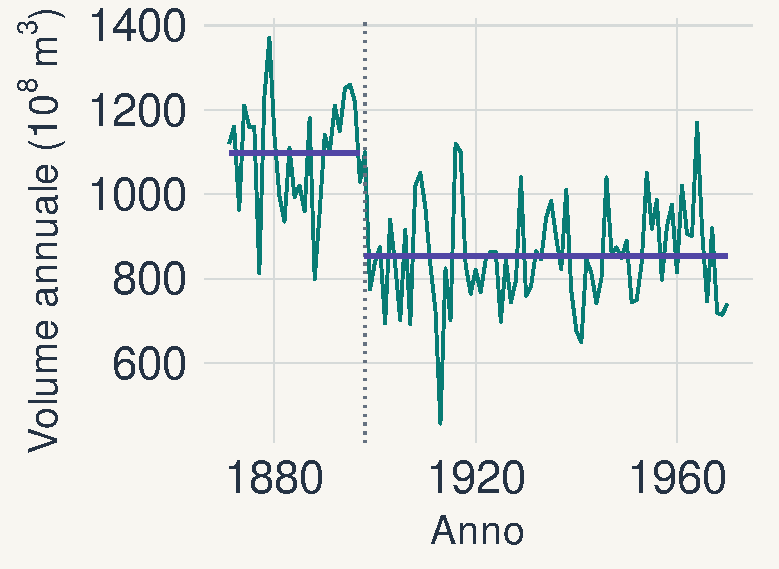
\includegraphics[width=\linewidth,height=6.15cm,keepaspectratio]{Figure/F01.pdf}\par}
\PSmall{Cento volumi annuali. Segmenti viola: medie dei due periodi; linea verticale: soglia dichiarata del 1898.}
}};
\node[anchor=north west,inner sep=0] at([xshift=10.85cm,yshift=-2.12cm]current page.north west){\Colonna{8.16cm}{\PBody{La linea unisce anni consecutivi e mostra la variabilità attorno ai due livelli medi, rappresentati dai segmenti viola. La separazione dichiarata compare insieme alle fluttuazioni che rimangono entro ciascun periodo. In questo modo, un confronto fra medie resta collegato alla storia osservata e alle possibili strutture residue. Il grafico non identifica il momento di un intervento causale né dimostra che ogni anno successivo appartenga a un regime fisico omogeneo; fornisce la descrizione sulla quale verrà costruito il modello semplificato.}
}};
\end{tikzpicture}\end{frame}

\begin{frame}[plain]\hypertarget{slide8}{}
\bookmark[level=1,page=8]{Distribuzioni marginali e diversa durata dei periodi}
\begin{tikzpicture}[remember picture,overlay]
\PilotChrome{{\fontsize{15.3}{19}\selectfont Distribuzioni marginali e diversa durata dei periodi}}{SERIE STORICA E CONTRASTO DICHIARATO}{8}{Il confronto delle distribuzioni conserva le numerosità e viene letto insieme all’ordine temporale.}
\node[anchor=north west,inner sep=0] at([xshift=.96cm,yshift=-2.12cm]current page.north west){\Colonna{9.40cm}{{\centering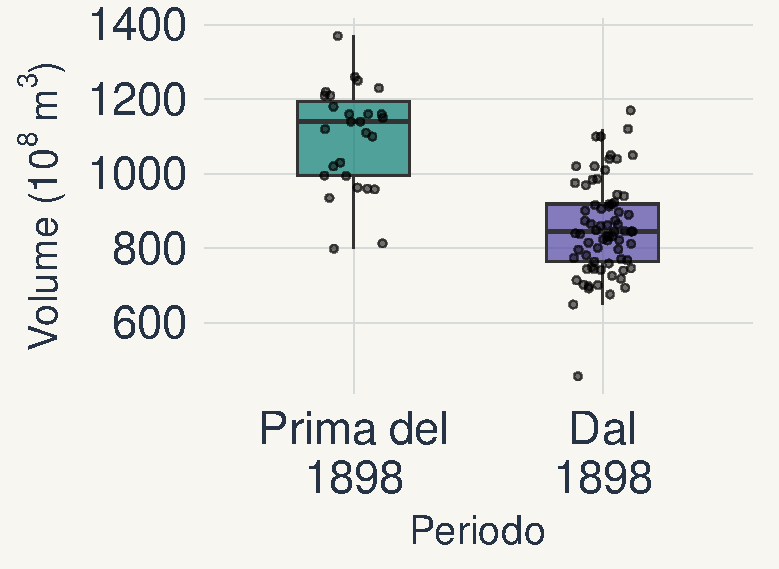
\includegraphics[width=\linewidth,height=6.15cm,keepaspectratio]{Figure/F02.pdf}\par}
\PSmall{Boxplot e osservazioni individuali. La dispersione orizzontale dei punti è soltanto grafica, con seme fissato.}
}};
\node[anchor=north west,inner sep=0] at([xshift=10.85cm,yshift=-2.12cm]current page.north west){\Colonna{8.16cm}{\PBody{Le distribuzioni per periodo riassumono posizione e dispersione dei volumi, conservando i punti individuali per mostrare le differenti numerosità. La separazione delle medie si accompagna a una sovrapposizione di valori, che impedisce di interpretare il contrasto come distinzione perfetta fra tutti gli anni. Il grafico marginale integra la serie temporale, dalla quale dipende l’esame dell’ordine e della persistenza. Le due rappresentazioni rispondono pertanto a esigenze complementari della descrizione, pur utilizzando gli stessi cento dati.}
}};
\end{tikzpicture}\end{frame}

\begin{frame}[plain]\hypertarget{slide9}{}
\bookmark[level=0,page=9]{Modello del livello e residui}
\bookmark[level=1,page=9]{La regressione codifica una differenza fra medie}
\begin{tikzpicture}[remember picture,overlay]
\PilotChrome{La regressione codifica una differenza fra medie}{MODELLO DEL LIVELLO E RESIDUI}{9}{Il significato di un coefficiente dipende dalla codifica del modello e dall’unità della risposta.}
\node[anchor=north west,inner sep=0] at([xshift=.96cm,yshift=-2.12cm]current page.north west){\Colonna{9.40cm}{\PBody{Il modello comprende un’intercetta e l’indicatore del secondo periodo. Per un anno iniziale, il valore atteso è l’intercetta; per un anno successivo è la somma dei due coefficienti. La pendenza dell’indicatore coincide quindi con la differenza fra medie, mentre il termine residuo raccoglie gli scostamenti annuali. La specificazione assume un livello costante entro ciascun periodo. Eventuali tendenze interne o altre variazioni sistematiche della media richiederebbero una formulazione ulteriore, che una correzione della covarianza non introduce.}
\par\smallskip{\centering\adjustbox{max width=.98\linewidth}{$\displaystyle \begin{gathered}Y_t=\alpha+\beta D_t+\varepsilon_t,\qquad D_t=\mathbf1\{t\geq1898\}\\\widehat\beta=\overline Y_{1898:1970}-\overline Y_{1871:1897}\end{gathered}$}\par\smallskip}
}};
\node[anchor=north west,inner sep=0] at([xshift=10.85cm,yshift=-2.12cm]current page.north west){\Colonna{8.16cm}{\PInfo{$Y_t$: volume annuale in $10^8$ m³; $\alpha$: livello iniziale; $\beta$: differenza dal 1898; $\varepsilon_t$: scarto a media nulla. Le barre indicano medie nei periodi riportati. Il codice confronta il coefficiente di lm con la differenza diretta. L’equivalenza verifica il calcolo; l’adeguatezza del modello richiede serie e residui.}
}};
\end{tikzpicture}\end{frame}

\begin{frame}[plain]\hypertarget{slide10}{}
\bookmark[level=1,page=10]{Grandezza assoluta e variazione relativa}
\begin{tikzpicture}[remember picture,overlay]
\PilotChrome{Grandezza assoluta e variazione relativa}{MODELLO DEL LIVELLO E RESIDUI}{10}{Una percentuale mantiene significato soltanto se il suo denominatore resta esplicito.}
\node[anchor=north west,inner sep=0] at([xshift=.96cm,yshift=-2.12cm]current page.north west){\Colonna{9.40cm}{{\centering\resizebox{0.90\linewidth}{!}{\begin{tikzpicture}[x=1cm,y=-.87cm,every node/.style={font=\fontsize{12.2}{15}\selectfont,text=Ink},arr/.style={-{Stealth[length=2mm]},line width=.8pt,draw=Classical}]\path[use as bounding box] (0,0) rectangle (7.45,6.2);
\draw[draw=Classical,fill=Classical!8,rounded corners=2pt,line width=.7pt] (0.6,0.8) rectangle (6.8,2.2);
\node[anchor=center,text=Ink,font=\fontsize{14}{15}\selectfont,text width=5.8cm,align=center] at (3.7,1.5) {Contrasto assoluto: -244,27};
\draw[arr,draw=Classical] (3.7,2.4)--(3.7,3.2);
\draw[draw=Quantum,fill=Quantum!8,rounded corners=2pt,line width=.7pt] (0.6,3.4) rectangle (6.8,4.8);
\node[anchor=center,text=Ink,font=\fontsize{13}{15}\selectfont,text width=5.8cm,align=center] at (3.7,4.1) {Variazione relativa: -22,25\%};
\node[anchor=center,text=Ink,font=\fontsize{11.5}{15}\selectfont,text width=6.5cm,align=center] at (3.7,5.6) {Denominatore: media del periodo iniziale};

\end{tikzpicture}}\par}
\PSmall{$\hat\beta$: media 1898–1970 meno media 1871–1897; $\bar Y_{1871:1897}$: media iniziale. $\hat r$ è espresso in percentuale.}
}};
\node[anchor=north west,inner sep=0] at([xshift=10.85cm,yshift=-2.12cm]current page.north west){\Colonna{8.16cm}{\PBody{Le medie dei due periodi sono rispettivamente 1097,67 e 853,40, nella scala di centinaia di milioni di metri cubi. La differenza stimata è -244,27, pari a una variazione del -22,25\% rispetto alla media iniziale. Il denominatore della percentuale viene dichiarato perché un confronto rispetto alla media successiva produrrebbe un valore diverso. Queste quantità descrivono la serie disponibile; la loro interpretazione probabilistica dipende dalle ipotesi sui processi annuali e dalla costruzione del riferimento inferenziale.}
\par\smallskip{\centering\adjustbox{max width=.98\linewidth}{$\displaystyle \widehat r=100\frac{\widehat\beta}{\overline Y_{1871:1897}}$}\par\smallskip}
}};
\end{tikzpicture}\end{frame}

\begin{frame}[plain]\hypertarget{slide11}{}
\bookmark[level=1,page=11]{L’intervallo classico come riferimento condizionato}
\begin{tikzpicture}[remember picture,overlay]
\PilotChrome{{\fontsize{15.3}{19}\selectfont L’intervallo classico come riferimento condizionato}}{MODELLO DEL LIVELLO E RESIDUI}{11}{Il riferimento classico va letto attraverso le ipotesi che giustificano il suo errore standard.}
\node[anchor=north west,inner sep=0] at([xshift=.96cm,yshift=-2.12cm]current page.north west){\Colonna{9.40cm}{\PBody{L’intervallo t della regressione utilizza una varianza residua comune e novantotto gradi di libertà. La sua interpretazione esatta richiede errori indipendenti, gaussiani e con varianza costante, oltre a una media correttamente specificata. L’indipendenza va esaminata attraverso l’ordine delle osservazioni. Il progetto conserva questo intervallo come riferimento esplicito, rispetto al quale valutare l’effetto di una diversa stima della covarianza, mantenendo invariata la stima del contrasto.}
\par\smallskip{\centering\adjustbox{max width=.98\linewidth}{$\displaystyle \begin{gathered}\widehat{\mathrm{Var}}_{iid}(\widehat\beta)=s^2\left(\frac1{27}+\frac1{73}\right)\\IC_{iid}=\widehat\beta\pm t_{0{,}975;98}\,SE_{iid}\end{gathered}$}\par\smallskip}
}};
\node[anchor=north west,inner sep=0] at([xshift=10.85cm,yshift=-2.12cm]current page.north west){\Colonna{8.16cm}{\PInfo{$s^2=\sum_t\hat e_t^2/98$, con $\hat e_t$ residuo annuale; SE è la radice della varianza stimata. $t_{0,975;98}\simeq1,984$ è il quantile t. Le numerosità sono 27 e 73. L’indipendenza riguarda la distribuzione congiunta degli errori: cento righe non garantiscono l’informazione di cento contributi indipendenti.}
}};
\end{tikzpicture}\end{frame}

\begin{frame}[plain]\hypertarget{slide12}{}
\bookmark[level=1,page=12]{I residui vengono riportati agli anni}
\begin{tikzpicture}[remember picture,overlay]
\PilotChrome{I residui vengono riportati agli anni}{MODELLO DEL LIVELLO E RESIDUI}{12}{Le proprietà algebriche dei residui devono essere distinte dalle ipotesi sul processo temporale.}
\node[anchor=north west,inner sep=0] at([xshift=.96cm,yshift=-2.12cm]current page.north west){\Colonna{9.40cm}{{\centering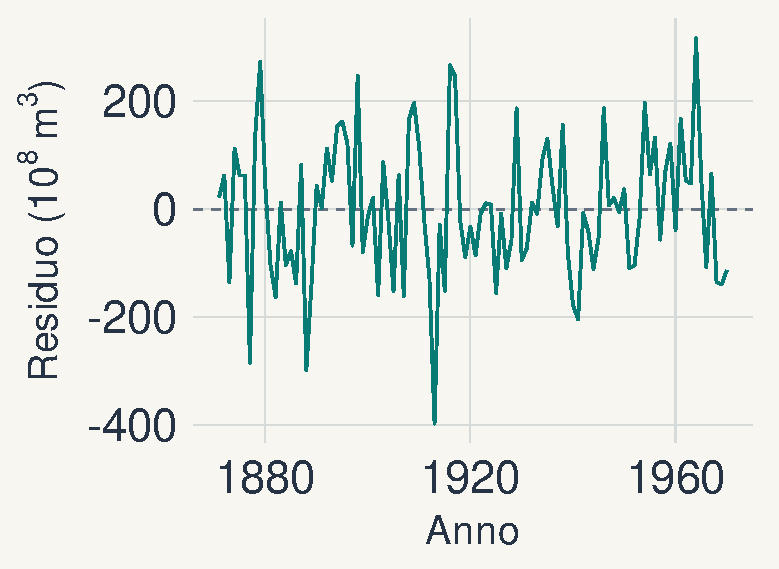
\includegraphics[width=\linewidth,height=6.15cm,keepaspectratio]{Figure/F03.pdf}\par}
\PSmall{Residui del modello a due livelli, ordinati per anno. Il riferimento orizzontale corrisponde allo scostamento nullo.}
}};
\node[anchor=north west,inner sep=0] at([xshift=10.85cm,yshift=-2.12cm]current page.north west){\Colonna{8.16cm}{\PBody{Sottraendo a ogni anno la media del proprio periodo si ottengono i residui del modello. La loro rappresentazione temporale permette di riconoscere sequenze persistenti, episodi estremi e possibili variazioni del livello rimaste nella specificazione. La somma dei residui entro ciascun periodo è nulla per costruzione, mentre l’assenza di dipendenza seriale costituisce una proprietà diversa. La diagnosi interpreta quindi ciò che la regressione lascia nella sequenza, evitando di attribuire al semplice centramento una giustificazione dell’indipendenza.}
}};
\end{tikzpicture}\end{frame}

\begin{frame}[plain]\hypertarget{slide13}{}
\bookmark[level=1,page=13]{L’ACF descrive la memoria residua}
\begin{tikzpicture}[remember picture,overlay]
\PilotChrome{L’ACF descrive la memoria residua}{MODELLO DEL LIVELLO E RESIDUI}{13}{L’ACF sostiene una diagnosi della dipendenza e richiede una lettura coerente con il modello della media.}
\node[anchor=north west,inner sep=0] at([xshift=.96cm,yshift=-2.12cm]current page.north west){\Colonna{9.40cm}{{\centering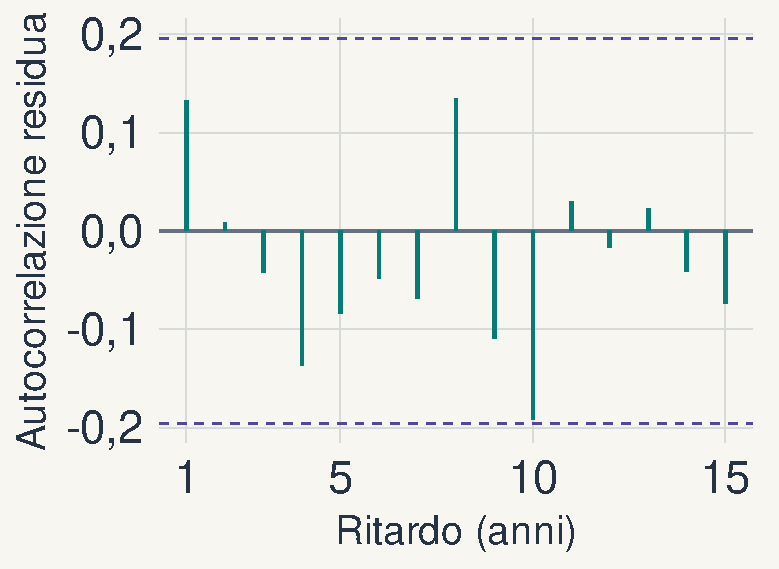
\includegraphics[width=\linewidth,height=6.15cm,keepaspectratio]{Figure/F04.pdf}\par}
\PSmall{$\hat e_t$: residuo centrato; n = 100; h: ritardo in anni. Bande puntuali $\pm1,96/\sqrt{100}$, senza correzione multipla.}
}};
\node[anchor=north west,inner sep=0] at([xshift=10.85cm,yshift=-2.12cm]current page.north west){\Colonna{8.16cm}{\PBody{L’autocorrelazione confronta residui separati da uno o più anni e riassume la persistenza lineare alle diverse distanze temporali. Le bande tratteggiate indicano il riferimento approssimativo di rumore bianco, calcolato come più o meno 1,96 diviso la radice di cento. Ogni banda riguarda una singola correlazione e non fornisce una verifica simultanea delle quindici barre. La lettura considera anche il disegno complessivo delle correlazioni e la possibilità che una struttura della media ancora omessa produca persistenza apparente.}
\par\smallskip{\centering\adjustbox{max width=.98\linewidth}{$\displaystyle \widehat\rho(h)=\frac{\sum_{t=h+1}^{n}\widehat e_t\widehat e_{t-h}}{\sum_{t=1}^{n}\widehat e_t^2}$}\par\smallskip}
}};
\end{tikzpicture}\end{frame}

\begin{frame}[plain]\hypertarget{slide14}{}
\bookmark[level=0,page=14]{Covarianza HAC e analisi di sensibilità}
\bookmark[level=1,page=14]{La dipendenza entra nella covarianza delle somme}
\begin{tikzpicture}[remember picture,overlay]
\PilotChrome{La dipendenza entra nella covarianza delle somme}{COVARIANZA HAC E ANALISI DI SENSIBILITÀ}{14}{La dipendenza modifica l’informazione contenuta nella somma attraverso le covarianze fra osservazioni.}
\node[anchor=north west,inner sep=0] at([xshift=.96cm,yshift=-2.12cm]current page.north west){\Colonna{9.40cm}{{\centering\resizebox{0.90\linewidth}{!}{\begin{tikzpicture}[x=1cm,y=-.87cm,every node/.style={font=\fontsize{12.2}{15}\selectfont,text=Ink},arr/.style={-{Stealth[length=2mm]},line width=.8pt,draw=Classical}]\path[use as bounding box] (0,0) rectangle (7.45,6.2);
\draw[draw=Quantum,fill=Quantum!8,rounded corners=2pt,line width=.7pt] (0.7,0.8) rectangle (1.4,1.45);
\draw[draw=Quantum,fill=Quantum!8,rounded corners=2pt,line width=.7pt] (1.45,0.8) rectangle (2.15,1.45);
\draw[draw=Rule,fill=Rule!8,rounded corners=2pt,line width=.7pt] (2.2,0.8) rectangle (2.9,1.45);
\draw[draw=Rule,fill=Rule!8,rounded corners=2pt,line width=.7pt] (2.95,0.8) rectangle (3.65,1.45);
\draw[draw=Rule,fill=Rule!8,rounded corners=2pt,line width=.7pt] (3.7,0.8) rectangle (4.4,1.45);
\draw[draw=Rule,fill=Rule!8,rounded corners=2pt,line width=.7pt] (4.45,0.8) rectangle (5.15,1.45);
\draw[draw=Quantum,fill=Quantum!8,rounded corners=2pt,line width=.7pt] (0.7,1.5) rectangle (1.4,2.15);
\draw[draw=Quantum,fill=Quantum!8,rounded corners=2pt,line width=.7pt] (1.45,1.5) rectangle (2.15,2.15);
\draw[draw=Quantum,fill=Quantum!8,rounded corners=2pt,line width=.7pt] (2.2,1.5) rectangle (2.9,2.15);
\draw[draw=Rule,fill=Rule!8,rounded corners=2pt,line width=.7pt] (2.95,1.5) rectangle (3.65,2.15);
\draw[draw=Rule,fill=Rule!8,rounded corners=2pt,line width=.7pt] (3.7,1.5) rectangle (4.4,2.15);
\draw[draw=Rule,fill=Rule!8,rounded corners=2pt,line width=.7pt] (4.45,1.5) rectangle (5.15,2.15);
\draw[draw=Rule,fill=Rule!8,rounded corners=2pt,line width=.7pt] (0.7,2.2) rectangle (1.4,2.8499999999999996);
\draw[draw=Quantum,fill=Quantum!8,rounded corners=2pt,line width=.7pt] (1.45,2.2) rectangle (2.15,2.8499999999999996);
\draw[draw=Quantum,fill=Quantum!8,rounded corners=2pt,line width=.7pt] (2.2,2.2) rectangle (2.9,2.8499999999999996);
\draw[draw=Quantum,fill=Quantum!8,rounded corners=2pt,line width=.7pt] (2.95,2.2) rectangle (3.65,2.8499999999999996);
\draw[draw=Rule,fill=Rule!8,rounded corners=2pt,line width=.7pt] (3.7,2.2) rectangle (4.4,2.8499999999999996);
\draw[draw=Rule,fill=Rule!8,rounded corners=2pt,line width=.7pt] (4.45,2.2) rectangle (5.15,2.8499999999999996);
\draw[draw=Rule,fill=Rule!8,rounded corners=2pt,line width=.7pt] (0.7,2.8999999999999995) rectangle (1.4,3.55);
\draw[draw=Rule,fill=Rule!8,rounded corners=2pt,line width=.7pt] (1.45,2.8999999999999995) rectangle (2.15,3.55);
\draw[draw=Quantum,fill=Quantum!8,rounded corners=2pt,line width=.7pt] (2.2,2.8999999999999995) rectangle (2.9,3.55);
\draw[draw=Quantum,fill=Quantum!8,rounded corners=2pt,line width=.7pt] (2.95,2.8999999999999995) rectangle (3.65,3.55);
\draw[draw=Quantum,fill=Quantum!8,rounded corners=2pt,line width=.7pt] (3.7,2.8999999999999995) rectangle (4.4,3.55);
\draw[draw=Rule,fill=Rule!8,rounded corners=2pt,line width=.7pt] (4.45,2.8999999999999995) rectangle (5.15,3.55);
\draw[draw=Rule,fill=Rule!8,rounded corners=2pt,line width=.7pt] (0.7,3.5999999999999996) rectangle (1.4,4.25);
\draw[draw=Rule,fill=Rule!8,rounded corners=2pt,line width=.7pt] (1.45,3.5999999999999996) rectangle (2.15,4.25);
\draw[draw=Rule,fill=Rule!8,rounded corners=2pt,line width=.7pt] (2.2,3.5999999999999996) rectangle (2.9,4.25);
\draw[draw=Quantum,fill=Quantum!8,rounded corners=2pt,line width=.7pt] (2.95,3.5999999999999996) rectangle (3.65,4.25);
\draw[draw=Quantum,fill=Quantum!8,rounded corners=2pt,line width=.7pt] (3.7,3.5999999999999996) rectangle (4.4,4.25);
\draw[draw=Quantum,fill=Quantum!8,rounded corners=2pt,line width=.7pt] (4.45,3.5999999999999996) rectangle (5.15,4.25);
\draw[draw=Rule,fill=Rule!8,rounded corners=2pt,line width=.7pt] (0.7,4.3) rectangle (1.4,4.95);
\draw[draw=Rule,fill=Rule!8,rounded corners=2pt,line width=.7pt] (1.45,4.3) rectangle (2.15,4.95);
\draw[draw=Rule,fill=Rule!8,rounded corners=2pt,line width=.7pt] (2.2,4.3) rectangle (2.9,4.95);
\draw[draw=Rule,fill=Rule!8,rounded corners=2pt,line width=.7pt] (2.95,4.3) rectangle (3.65,4.95);
\draw[draw=Quantum,fill=Quantum!8,rounded corners=2pt,line width=.7pt] (3.7,4.3) rectangle (4.4,4.95);
\draw[draw=Quantum,fill=Quantum!8,rounded corners=2pt,line width=.7pt] (4.45,4.3) rectangle (5.15,4.95);
\node[anchor=center,text=Ink,font=\fontsize{11.5}{15}\selectfont,text width=6.5cm,align=center] at (3.7,0.45) {Covarianze fra contributi temporali};
\node[anchor=center,text=Ink,font=\fontsize{11}{15}\selectfont,text width=6.7cm,align=center] at (3.7,6) {Diagonale: varianze; bande: ritardi vicini.};

\end{tikzpicture}}\par}
\PSmall{$Z_t$: contributo casuale con varianza finita. HAC ammette eteroschedasticità e autocorrelazione sotto ipotesi asintotiche.}
}};
\node[anchor=north west,inner sep=0] at([xshift=10.85cm,yshift=-2.12cm]current page.north west){\Colonna{8.16cm}{\PBody{Quando gli errori sono correlati, la varianza di una somma comprende anche le covarianze fra termini distinti. La matrice HAC applica questo principio ai contributi della regressione, conservando i prodotti fra residui e righe della matrice del modello a diversi ritardi. La stima OLS resta invariata, mentre cambia la covarianza che ne descrive l’incertezza. La costruzione richiede condizioni di dipendenza debole e un modello della media adeguato; il suo carattere asintotico deve rimanere esplicito anche con cento osservazioni.}
\par\smallskip{\centering\adjustbox{max width=.98\linewidth}{$\displaystyle \mathrm{Var}\!\left(\sum_t Z_t\right)=\sum_t\mathrm{Var}(Z_t)+2\sum_{s<t}\mathrm{Cov}(Z_s,Z_t)$}\par\smallskip}
}};
\end{tikzpicture}\end{frame}

\begin{frame}[plain]\hypertarget{slide15}{}
\bookmark[level=1,page=15]{Pesi di Bartlett e ritardo massimo dichiarato}
\begin{tikzpicture}[remember picture,overlay]
\PilotChrome{Pesi di Bartlett e ritardo massimo dichiarato}{COVARIANZA HAC E ANALISI DI SENSIBILITÀ}{15}{Il ritardo massimo è una scelta del protocollo, della quale viene esaminata la sensibilità.}
\node[anchor=north west,inner sep=0] at([xshift=.96cm,yshift=-2.12cm]current page.north west){\Colonna{9.40cm}{\PBody{Si indicano con u i prodotti fra la riga del modello e il residuo corrispondente. La matrice interna della covarianza somma i prodotti contemporanei e quelli ritardati, assegnando a questi ultimi pesi di Bartlett decrescenti. Il progetto fissa inizialmente un ritardo massimo di tre anni, senza prewhitening. La figura confronta i pesi per tre e dieci anni, rendendo visibile come la scelta determini quali associazioni residue entrino nel calcolo e con quale contributo.}
\par\smallskip{\centering\adjustbox{max width=.98\linewidth}{$\displaystyle \begin{gathered}u_t=x_t\widehat e_t,\quad G_h=\sum_{t=h+1}^{n}u_tu_{t-h}^{T}\\S_L=G_0+\sum_{h=1}^{L}\left(1-\frac{h}{L+1}\right)(G_h+G_h^T)\end{gathered}$}\par\smallskip}
}};
\node[anchor=north west,inner sep=0] at([xshift=10.85cm,yshift=-2.12cm]current page.north west){\Colonna{8.16cm}{{\centering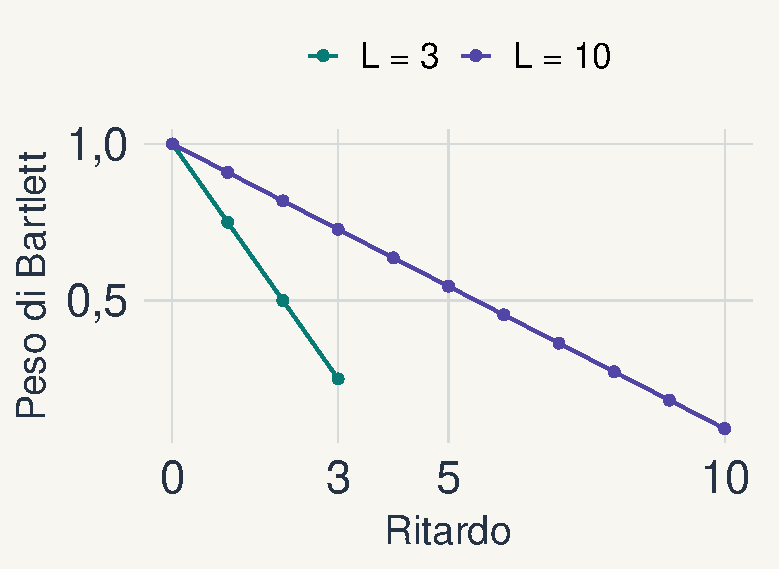
\includegraphics[width=\linewidth,height=5.3cm,keepaspectratio]{Figure/F08.pdf}\par}
\PSmall{$x_t=(1,D_t)^T$, con $D_t=1$ dal 1898; $\hat e_t$: residuo; n = 100. h: ritardo; L: massimo incluso. T indica trasposizione.}
}};
\end{tikzpicture}\end{frame}

\begin{frame}[plain]\hypertarget{slide16}{}
\bookmark[level=1,page=16]{Dalla matrice interna all’intervallo asintotico}
\begin{tikzpicture}[remember picture,overlay]
\PilotChrome{Dalla matrice interna all’intervallo asintotico}{COVARIANZA HAC E ANALISI DI SENSIBILITÀ}{16}{Formula, correzione finita, ritardo e distribuzione di riferimento devono essere riportati insieme.}
\node[anchor=north west,inner sep=0] at([xshift=.96cm,yshift=-2.12cm]current page.north west){\Colonna{9.40cm}{\PBody{La matrice interna viene trasformata mediante l’inversa di X trasposta X e moltiplicata per il fattore cento diviso novantotto. Questa convenzione corrisponde alla correzione finita n diviso n meno k, con due coefficienti stimati. L’errore standard della differenza è la radice dell’elemento diagonale corrispondente alla pendenza. L’intervallo adotta il quantile normale 1,96 e rimane asintotico: la correzione finita non lo trasforma in un intervallo esatto per una serie di lunghezza limitata.}
\par\smallskip{\centering\adjustbox{max width=.98\linewidth}{$\displaystyle \begin{gathered}\widehat V_{HAC}=\frac{n}{n-k}(X^TX)^{-1}S_L(X^TX)^{-1}\\IC_{HAC}=\widehat\beta\pm1{,}96\sqrt{[\widehat V_{HAC}]_{22}}\end{gathered}$}\par\smallskip}
}};
\node[anchor=north west,inner sep=0] at([xshift=10.85cm,yshift=-2.12cm]current page.north west){\Colonna{8.16cm}{\PInfo{X ha colonne 1 e indicatore del periodo dal 1898; n = 100, k = 2. $S_L$ somma i prodotti dei vettori regressore × residuo, contemporanei e ritardati, con pesi di Bartlett fino a L = 3. L’elemento 22 riguarda la differenza $\beta$. R/covarianze.R implementa la formula; il collaudo verifica simmetria e concordanza con un secondo calcolo.}
}};
\end{tikzpicture}\end{frame}

\begin{frame}[plain]\hypertarget{slide17}{}
\bookmark[level=1,page=17]{Il calcolo mantiene separati stima e incertezza}
\begin{tikzpicture}[remember picture,overlay]
\PilotChrome{Il calcolo mantiene separati stima e incertezza}{COVARIANZA HAC E ANALISI DI SENSIBILITÀ}{17}{La variante della covarianza cambia l’incertezza attribuita al medesimo contrasto OLS.}
\node[anchor=north west,inner sep=0] at([xshift=.96cm,yshift=-2.12cm]current page.north west){\Colonna{9.40cm}{\PBody{Il frammento stima il modello una sola volta e passa matrice del disegno e residui alla funzione HAC. Il contrasto rimane -244,27, mentre l’errore standard HAC è circa 31,70. L’intervallo normale corrispondente si estende da -306,39 a -182,15, nella scala dei volumi annuali. La separazione fra adattamento e covarianza rende controllabile quale componente dell’analisi sia stata modificata e impedisce di confondere una maggiore precisione numerica con un cambiamento della stima.}
}};
\node[anchor=north west,inner sep=0] at([xshift=10.85cm,yshift=-2.12cm]current page.north west){\Colonna{8.16cm}{\begin{tcolorbox}[enhanced,arc=1.7mm,boxrule=.6pt,colback=white,colframe=Classical!60!Navy,colbacktitle=Navy,coltitle=white,fonttitle=\bfseries\small,title={R · calcolo riproducibile},left=1.7mm,right=1.3mm,top=1.1mm,bottom=1.1mm,before skip=1mm,after skip=1.0mm]\lstinputlisting[style=GeoR,language=R,basicstyle=\ttfamily\fontsize{8.6}{11.4}\selectfont]{Codice/HAC.R}\end{tcolorbox}
\PLabel{Risultato in R}
\begin{tcolorbox}[colback=GeoTint,colframe=Rule,boxrule=.5pt,arc=1.4mm,left=2mm,right=1mm,top=1mm,bottom=1mm]{\fontsize{8.4}{10.9}\selectfont\ttfamily \mbox{\ \ \ \ \ post\ \ \ \ \ \ post\ }\\\mbox{-306.3933\ -182.1456\ }}\end{tcolorbox}
}};
\end{tikzpicture}\end{frame}

\begin{frame}[plain]\hypertarget{slide18}{}
\bookmark[level=1,page=18]{Intervalli riferiti alla stessa differenza}
\begin{tikzpicture}[remember picture,overlay]
\PilotChrome{Intervalli riferiti alla stessa differenza}{COVARIANZA HAC E ANALISI DI SENSIBILITÀ}{18}{La robustezza a una specificazione riguarda le varianti effettivamente esaminate.}
\node[anchor=north west,inner sep=0] at([xshift=.96cm,yshift=-2.12cm]current page.north west){\Colonna{9.40cm}{{\centering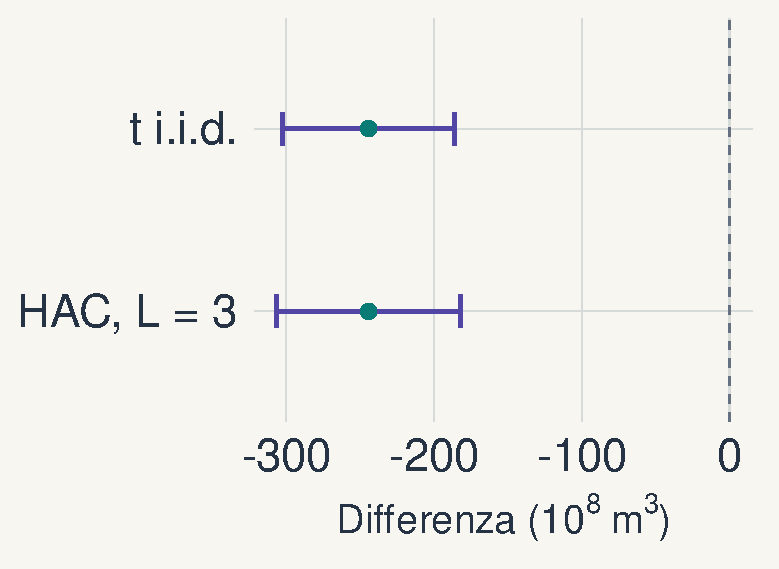
\includegraphics[width=\linewidth,height=6.15cm,keepaspectratio]{Figure/F05.pdf}\par}
\PSmall{Intervallo t i.i.d. e intervallo normale HAC con L = 3. Unità: centinaia di milioni di metri cubi.}
}};
\node[anchor=north west,inner sep=0] at([xshift=10.85cm,yshift=-2.12cm]current page.north west){\Colonna{8.16cm}{\PBody{Le due costruzioni vengono rappresentate sulla stessa scala e condividono la stima centrale. La loro diversa ampiezza dipende dalle ipotesi sulla struttura degli errori e dalla formula di covarianza. Un intervallo HAC può essere più ampio o più stretto di quello classico, poiché il risultato dipende da segno e intensità delle covarianze stimate. L’argomento si concentra sulla stabilità della conclusione entro le specificazioni dichiarate, mantenendo distinta questa sensibilità dall’incertezza relativa alla scelta storica della soglia.}
}};
\end{tikzpicture}\end{frame}

\begin{frame}[plain]\hypertarget{slide19}{}
\bookmark[level=1,page=19]{Sensibilità alla memoria inclusa nel calcolo}
\begin{tikzpicture}[remember picture,overlay]
\PilotChrome{Sensibilità alla memoria inclusa nel calcolo}{COVARIANZA HAC E ANALISI DI SENSIBILITÀ}{19}{L’analisi di sensibilità documenta le conseguenze delle scelte mantenendo visibili tutte le varianti.}
\node[anchor=north west,inner sep=0] at([xshift=.96cm,yshift=-2.12cm]current page.north west){\Colonna{9.40cm}{{\centering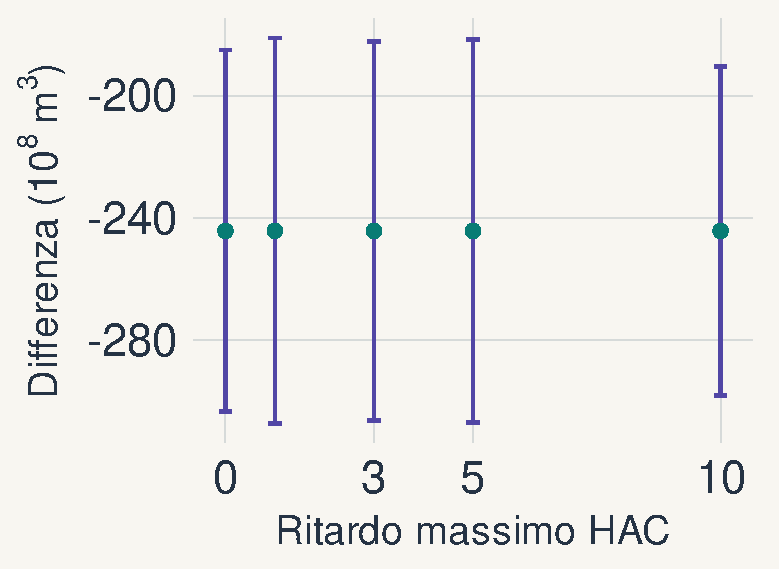
\includegraphics[width=\linewidth,height=6.15cm,keepaspectratio]{Figure/F06.pdf}\par}
\PSmall{Stima OLS comune e intervalli HAC su una griglia dichiarata di ritardi massimi.}
}};
\node[anchor=north west,inner sep=0] at([xshift=10.85cm,yshift=-2.12cm]current page.north west){\Colonna{8.16cm}{\PBody{La griglia dei ritardi massimi comprende zero, uno, tre, cinque e dieci anni. Ogni variante mantiene gli stessi dati e lo stesso modello della media, modificando soltanto la quantità di dipendenza residua inclusa nella covarianza. Il caso zero conserva una correzione per eteroschedasticità e omette i prodotti ritardati; gli altri casi aggiungono contributi pesati. Presentare l’intera griglia permette di discutere l’incertezza senza selezionare a posteriori il ritardo che favorisca una conclusione desiderata.}
}};
\end{tikzpicture}\end{frame}

\begin{frame}[plain]\hypertarget{slide20}{}
\bookmark[level=1,page=20]{Sensibilità alla collocazione della separazione}
\begin{tikzpicture}[remember picture,overlay]
\PilotChrome{Sensibilità alla collocazione della separazione}{COVARIANZA HAC E ANALISI DI SENSIBILITÀ}{20}{La ricerca della soglia e la stima condizionata a una soglia sono problemi inferenziali differenti.}
\node[anchor=north west,inner sep=0] at([xshift=.96cm,yshift=-2.12cm]current page.north west){\Colonna{9.40cm}{{\centering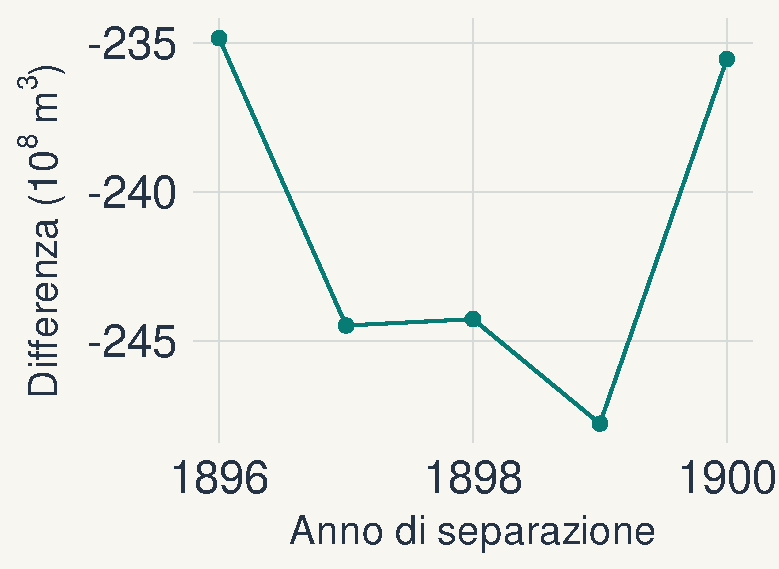
\includegraphics[width=\linewidth,height=6.15cm,keepaspectratio]{Figure/F07.pdf}\par}
\PSmall{Differenza fra periodi per cinque soglie vicine. Confronto descrittivo, distinto da una ricerca inferenziale della rottura.}
}};
\node[anchor=north west,inner sep=0] at([xshift=10.85cm,yshift=-2.12cm]current page.north west){\Colonna{8.16cm}{\PBody{Spostando la soglia dal 1896 al 1900 si modifica l’assegnazione di pochi anni e si ricalcola la differenza fra medie. La figura descrive quanto il contrasto dipenda dalla collocazione precisa del confine entro questo intervallo storico. Le cinque stime utilizzano quasi tutti gli stessi dati e non costituiscono cinque conferme indipendenti. Un’analisi che cercasse automaticamente il punto di cambiamento richiederebbe un’inferenza capace di rappresentare la selezione della soglia e la sua incertezza.}
}};
\end{tikzpicture}\end{frame}

\begin{frame}[plain]\hypertarget{slide21}{}
\bookmark[level=0,page=21]{Interpretazione idrologica e consegna}
\bookmark[level=1,page=21]{La successione temporale lascia aperta la causa}
\begin{tikzpicture}[remember picture,overlay]
\PilotChrome{La successione temporale lascia aperta la causa}{INTERPRETAZIONE IDROLOGICA E CONSEGNA}{21}{L’attribuzione causale richiede un disegno e informazioni che il solo contrasto temporale non fornisce.}
\node[anchor=north west,inner sep=0] at([xshift=.96cm,yshift=-2.12cm]current page.north west){\Colonna{9.40cm}{{\centering\resizebox{0.90\linewidth}{!}{\begin{tikzpicture}[x=1cm,y=-.87cm,every node/.style={font=\fontsize{12.2}{15}\selectfont,text=Ink},arr/.style={-{Stealth[length=2mm]},line width=.8pt,draw=Classical}]\path[use as bounding box] (0,0) rectangle (7.45,6.2);
\draw[draw=Classical,fill=Classical!8,rounded corners=2pt,line width=.7pt] (0.5,0.6) rectangle (6.9,1.9);
\node[anchor=center,text=Ink,font=\fontsize{12.2}{15}\selectfont,text width=6cm,align=center] at (3.7,1.25) {Differenza osservata fra periodi};
\draw[arr,draw=Classical] (2,2.1)--(2,3);
\draw[arr,draw=Quantum] (5.4,2.1)--(5.4,3);
\draw[draw=Classical,fill=Classical!8,rounded corners=2pt,line width=.7pt] (0.4,3.2) rectangle (3.5,4.7);
\node[anchor=center,text=Ink,font=\fontsize{11.5}{15}\selectfont,text width=2.7cm,align=center] at (1.95,3.95) {Forzanti e interventi};
\draw[draw=Quantum,fill=Quantum!8,rounded corners=2pt,line width=.7pt] (3.9,3.2) rectangle (7,4.7);
\node[anchor=center,text=Ink,font=\fontsize{11.5}{15}\selectfont,text width=2.7cm,align=center] at (5.45,3.95) {Misura e copertura};
\node[anchor=center,text=Ink,font=\fontsize{11.5}{15}\selectfont,text width=6.7cm,align=center] at (3.7,5.6) {Confronto delle spiegazioni mediante dati ulteriori};

\end{tikzpicture}}\par}
}};
\node[anchor=north west,inner sep=0] at([xshift=10.85cm,yshift=-2.12cm]current page.north west){\Colonna{8.16cm}{\PBody{Il contrasto quantifica una differenza della serie e non identifica l’effetto di una specifica opera idraulica o forzante climatica. Per un’attribuzione occorrerebbero cronologie degli interventi, precipitazioni, informazioni sul bacino e metadati strumentali, oltre a una strategia che distingua spiegazioni concorrenti. La covarianza HAC riguarda l’incertezza del coefficiente sotto il modello e non sostituisce tali informazioni. La relazione conserva pertanto la conclusione descrittiva e formula le osservazioni aggiuntive necessarie a sostenere un’interpretazione fisica più specifica.}
}};
\end{tikzpicture}\end{frame}

\begin{frame}[plain]\hypertarget{slide22}{}
\bookmark[level=1,page=22]{Consegna: sostenere il contrasto e i suoi limiti}
\begin{tikzpicture}[remember picture,overlay]
\PilotChrome{Consegna: sostenere il contrasto e i suoi limiti}{INTERPRETAZIONE IDROLOGICA E CONSEGNA}{22}{La conclusione collega grandezza, incertezza, origine della soglia e limiti dell’attribuzione.}
\node[anchor=north west,inner sep=0] at([xshift=.96cm,yshift=-2.12cm]current page.north west){\Colonna{9.40cm}{\PBody{La relazione include serie storica, distribuzioni per periodo, contrasto con unità, residui, ACF e confronto degli intervalli. L’esercizio richiede di spiegare perché la stima rimanga invariata passando alla covarianza HAC, mentre la sua precisione cambi. Una risposta completa richiama la presenza dei prodotti ritardati nella varianza e mantiene esplicite le ipotesi asintotiche. Un secondo esercizio esamina l’effetto di una soglia scelta dopo aver osservato la serie, distinguendo questa selezione dalla sensibilità condizionata alle soglie dichiarate.}
}};
\node[anchor=north west,inner sep=0] at([xshift=10.85cm,yshift=-2.12cm]current page.north west){\Colonna{8.16cm}{\PInfo{R/P03\_figure.R produce figure, tabelle e risultati a partire da dati/progetti/nile.csv. La formulazione raccorda regressione, dipendenza temporale e inferenza sviluppate nei moduli M05, M07 e M09. La lettura della documentazione della fonte accompagna l’interpretazione delle unità e della soglia storica.}
}};
\end{tikzpicture}\end{frame}

\begin{frame}[plain]\hypertarget{slide23}{}
\bookmark[level=0,page=23]{Laboratori della spedizione}
\bookmark[level=1,page=23]{Tre fasi della spedizione nel laboratorio}
\begin{tikzpicture}[remember picture,overlay]
\PilotChrome{Tre fasi della spedizione nel laboratorio}{LABORATORI DELLA SPEDIZIONE}{23}{Gli esperimenti usano serie sintetiche; la conclusione sul caso resta quella ottenuta dai cento volumi.}
\node[anchor=north west,inner sep=0] at([xshift=.96cm,yshift=-2.12cm]current page.north west){\Colonna{9.40cm}{{\centering\resizebox{0.97\linewidth}{!}{\begin{tikzpicture}[x=1cm,y=1cm,every node/.style={font=\sffamily\fontsize{9.2}{11}\selectfont,text=Ink}]
\node[draw=Classical,fill=Classical,rounded corners=2mm,text=white,text width=2.45cm,align=flush center,minimum height=1.55cm,anchor=west,font=\sffamily\bfseries\fontsize{9.2}{11}\selectfont] (f0) at (0,0.00) {1. Leggere la serie};
\node[draw=Classical!60,fill=Classical!6,rounded corners=1.5mm,line width=.6pt,text width=2.8cm,align=flush center,minimum height=1.55cm,anchor=west] (e00) at (2.95,0.00) {Calendario e osservazioni mancanti\\[1pt]{\fontsize{7.6}{9}\selectfont\color{Muted}m09-calendario}};
\node[draw=Rule,fill=white,rounded corners=1.5mm,line width=.6pt,text width=2.8cm,align=flush center,minimum height=1.55cm,anchor=west] (e01) at (6.10,0.00) {Trend, stagionalità e media mobile\\[1pt]{\fontsize{7.6}{9}\selectfont\color{Muted}m09-smoothing}};
\draw[pEdge] (f0.east)--(e00.west);
\node[draw=Classical,fill=Classical,rounded corners=2mm,text=white,text width=2.45cm,align=flush center,minimum height=1.55cm,anchor=west,font=\sffamily\bfseries\fontsize{9.2}{11}\selectfont] (f1) at (0,-1.95) {2. Diagnosticare la dipendenza};
\draw[pEdge] (f0.south)--(f1.north);
\node[draw=Classical!60,fill=Classical!6,rounded corners=1.5mm,line width=.6pt,text width=2.8cm,align=flush center,minimum height=1.55cm,anchor=west] (e10) at (2.95,-1.95) {Ritardi e autocorrelazione\\[1pt]{\fontsize{7.6}{9}\selectfont\color{Muted}m09-autocorrelazione}};
\node[draw=Rule,fill=white,rounded corners=1.5mm,line width=.6pt,text width=2.8cm,align=flush center,minimum height=1.55cm,anchor=west] (e11) at (6.10,-1.95) {Trasformazione e differenziazione\\[1pt]{\fontsize{7.6}{9}\selectfont\color{Muted}m09-differenze}};
\draw[pEdge] (f1.east)--(e10.west);
\node[draw=Classical,fill=Classical,rounded corners=2mm,text=white,text width=2.45cm,align=flush center,minimum height=1.55cm,anchor=west,font=\sffamily\bfseries\fontsize{9.2}{11}\selectfont] (f2) at (0,-3.90) {3. Sostenere la conclusione};
\draw[pEdge] (f1.south)--(f2.north);
\node[draw=Classical!60,fill=Classical!6,rounded corners=1.5mm,line width=.6pt,text width=2.8cm,align=flush center,minimum height=1.55cm,anchor=west] (e20) at (2.95,-3.90) {Bootstrap a blocchi di una serie dipendente\\[1pt]{\fontsize{7.6}{9}\selectfont\color{Muted}m05-blocchi}};
\node[draw=Rule,fill=white,rounded corners=1.5mm,line width=.6pt,text width=2.8cm,align=flush center,minimum height=1.55cm,anchor=west] (e21) at (6.10,-3.90) {Effetto, intervallo ed evidenza\\[1pt]{\fontsize{7.6}{9}\selectfont\color{Muted}m06-relazione}};
\draw[pEdge] (f2.east)--(e20.west);
\end{tikzpicture}
}\par}
\PSmall{Fasi della spedizione. Il primo esperimento di ogni fase ha le pagine Scenario A e Confronto.}
}};
\node[anchor=north west,inner sep=0] at([xshift=10.85cm,yshift=-2.12cm]current page.north west){\Colonna{8.16cm}{\PBody{Gli esperimenti ripetono su dati sintetici tre passaggi della spedizione: leggere una serie con il suo calendario, diagnosticare la dipendenza fra osservazioni vicine, ricampionare una serie dipendente. Ogni fase ha uno scenario di partenza e un confronto con un solo parametro modificato.}
\vspace{.2cm}\PLabel{Altri esperimenti delle fasi}
\PLab{https://marzione00.github.io/Lab_Geo/\#laboratorio/m09-smoothing}{Trend, stagionalità e media mobile · m09-smoothing}
\PLab{https://marzione00.github.io/Lab_Geo/\#laboratorio/m09-differenze}{Trasformazione e differenziazione · m09-differenze}
\PLab{https://marzione00.github.io/Lab_Geo/\#laboratorio/m06-relazione}{Effetto, intervallo ed evidenza · m06-relazione}
}};
\end{tikzpicture}\end{frame}

\begin{frame}[plain]\hypertarget{slide24}{}
\bookmark[level=1,page=24]{Calendario e osservazioni mancanti}
\begin{tikzpicture}[remember picture,overlay]
\PilotChrome{Calendario e osservazioni mancanti}{LABORATORI DELLA SPEDIZIONE}{24}{Distinguere distanza temporale e posizione nella tabella.}
\node[anchor=north west,inner sep=0] at([xshift=.96cm,yshift=-2.12cm]current page.north west){\Colonna{9.40cm}{{\centering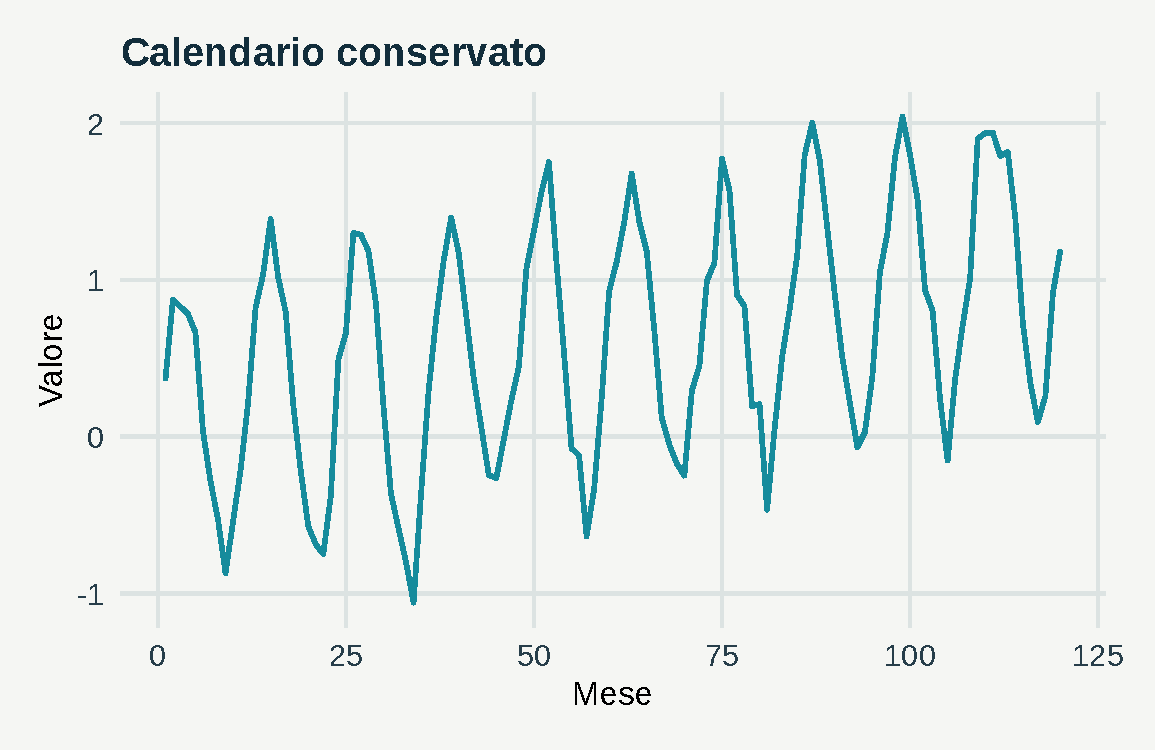
\includegraphics[width=\linewidth,height=5.0cm,keepaspectratio]{Esperimenti/m09-calendario-A.pdf}\par}
\PSmall{Mesi da escludere: 8. Seme: 17.}
\PSmall{$t_i$ è il mese della $i$-esima osservazione disponibile; $\Delta t_i$ è il tempo trascorso dalla precedente osservazione. In presenza di lacune, gli incrementi temporali possono essere maggiori di un mese.}
}};
\node[anchor=north west,inner sep=0] at([xshift=10.85cm,yshift=-2.12cm]current page.north west){\Colonna{8.16cm}{\PLabel{Scenario A · simulazione}
\PBody{La serie sintetica contiene una componente stagionale, un andamento di lungo periodo e rumore. Eliminando alcuni mesi si produce un insieme di osservazioni disponibili con intervalli temporali diseguali. Le date dei valori conservati rimangono note, consentendo di confrontare una rappresentazione che rispetta il calendario con una che utilizza soltanto la posizione nella tabella.}
\par\smallskip{\centering\adjustbox{max width=.98\linewidth}{$\displaystyle \Delta t_i=t_i-t_{i-1}$}\par\smallskip}
}};
\node[anchor=north east,inner sep=0] at([xshift=17.1cm,yshift=-12.04cm]current page.north west){\fontsize{7.7}{9}\selectfont \href{https://marzione00.github.io/Lab_Geo/\#laboratorio/m09-calendario}{\color{Classical}\bfseries Apri il laboratorio · m09-calendario}};
\end{tikzpicture}\end{frame}

\begin{frame}[plain]\hypertarget{slide25}{}
\bookmark[level=1,page=25]{Confronto | Calendario e osservazioni mancanti}
\begin{tikzpicture}[remember picture,overlay]
\PilotChrome{Confronto | Calendario e osservazioni mancanti}{LABORATORI DELLA SPEDIZIONE}{25}{L’indice di riga non sostituisce il calendario quando gli intervalli di osservazione sono irregolari.}
\node[anchor=north west,inner sep=0] at([xshift=.96cm,yshift=-2.12cm]current page.north west){\Colonna{9.40cm}{{\centering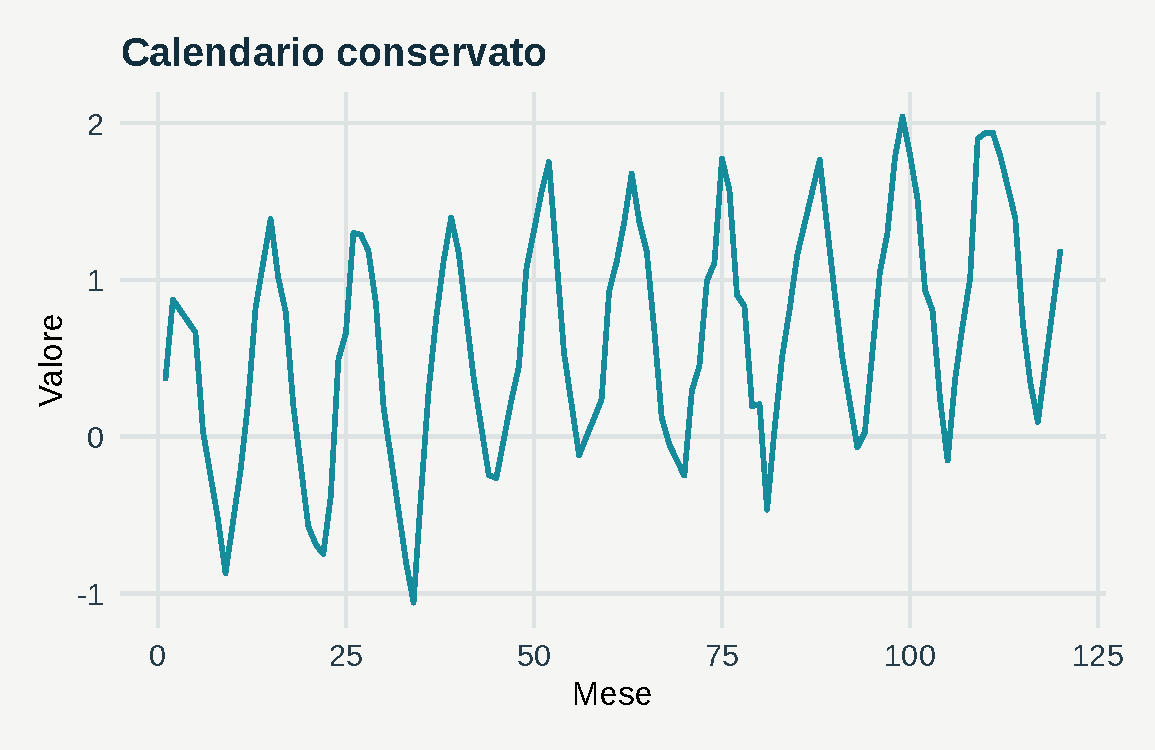
\includegraphics[width=\linewidth,height=5.6cm,keepaspectratio]{Esperimenti/m09-calendario-B.pdf}\par}
\PSmall{Mesi da escludere: 8 $\to$ 24. Tutti gli altri parametri e il seme sono fissi.}
}};
\node[anchor=north west,inner sep=0] at([xshift=10.85cm,yshift=-2.12cm]current page.north west){\Colonna{8.16cm}{\PLabel{Confronto fra gli scenari}
{\fontsize{10.2}{12.8}\selectfont\begin{tabular}{@{}>{\raggedright\arraybackslash}p{0.48\linewidth}@{\hspace{.13cm}}>{\raggedright\arraybackslash}p{0.224\linewidth}@{\hspace{.13cm}}>{\raggedright\arraybackslash}p{0.224\linewidth}@{}}\toprule Grandezza & A & B\\[2.3pt]
\midrule 
Osservazioni & 112 & 96\\[2.3pt]
Intervallo massimo fra osservazioni & 2 & 3\\[2.3pt]
\bottomrule\end{tabular}\par}
\vspace{.25cm}\PBody{Escludendo ventiquattro mesi le osservazioni scendono da 112 a 96 e l’intervallo massimo fra osservazioni consecutive passa da 2 a 3 mesi. Il calendario conserva la posizione delle lacune, che una numerazione delle righe nasconderebbe.}
}};
\node[anchor=north east,inner sep=0] at([xshift=17.1cm,yshift=-12.04cm]current page.north west){\fontsize{7.7}{9}\selectfont \href{https://marzione00.github.io/Lab_Geo/\#laboratorio/m09-calendario}{\color{Classical}\bfseries Apri il laboratorio · m09-calendario}};
\end{tikzpicture}\end{frame}

\begin{frame}[plain]\hypertarget{slide26}{}
\bookmark[level=1,page=26]{Ritardi e autocorrelazione}
\begin{tikzpicture}[remember picture,overlay]
\PilotChrome{Ritardi e autocorrelazione}{LABORATORI DELLA SPEDIZIONE}{26}{Collegare coppie temporali e dipendenza a un ritardo.}
\node[anchor=north west,inner sep=0] at([xshift=.96cm,yshift=-2.12cm]current page.north west){\Colonna{9.40cm}{{\centering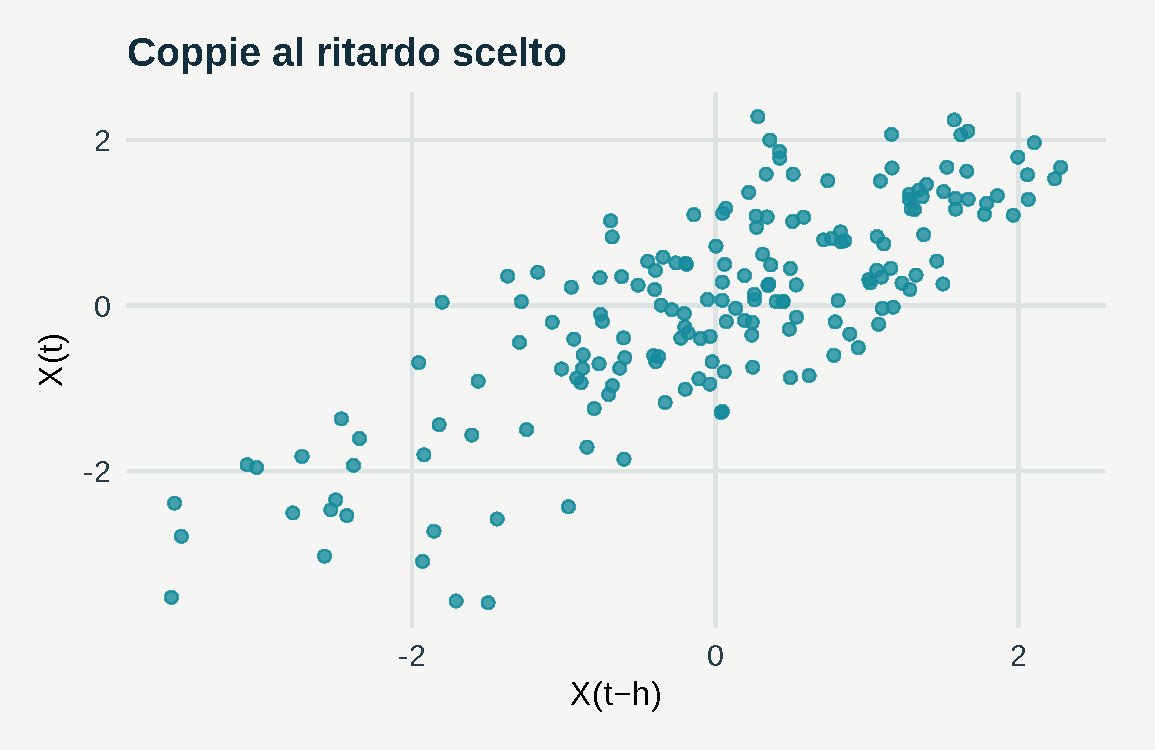
\includegraphics[width=\linewidth,height=5.0cm,keepaspectratio]{Esperimenti/m09-autocorrelazione-A.pdf}\par}
\PSmall{Parametro AR(1): 0,7. Seme: 17.}
\PSmall{$X_t$ è il valore al tempo $t$; $\phi$ è il coefficiente autoregressivo; $\varepsilon_t$ è l’innovazione indipendente. $\rho(h)$ è l’autocorrelazione teorica al ritardo $h$; qui $|\phi|<1$ e la varianza delle innovazioni è $1-\phi^2$.}
}};
\node[anchor=north west,inner sep=0] at([xshift=10.85cm,yshift=-2.12cm]current page.north west){\Colonna{8.16cm}{\PLabel{Scenario A · simulazione}
\PBody{Il processo autoregressivo viene inizializzato nella propria distribuzione stazionaria, con media nulla e varianza marginale unitaria. Ogni osservazione combina una frazione della precedente con una nuova innovazione indipendente. Il parametro autoregressivo determina intensità e segno della memoria, mentre il ritardo scelto stabilisce quali coppie vengono confrontate.}
\par\smallskip{\centering\adjustbox{max width=.98\linewidth}{$\displaystyle X_t=\phi X_{t-1}+\varepsilon_t,\quad\rho(h)=\phi^h$}\par\smallskip}
}};
\node[anchor=north east,inner sep=0] at([xshift=17.1cm,yshift=-12.04cm]current page.north west){\fontsize{7.7}{9}\selectfont \href{https://marzione00.github.io/Lab_Geo/\#laboratorio/m09-autocorrelazione}{\color{Classical}\bfseries Apri il laboratorio · m09-autocorrelazione}};
\end{tikzpicture}\end{frame}

\begin{frame}[plain]\hypertarget{slide27}{}
\bookmark[level=1,page=27]{Confronto | Ritardi e autocorrelazione}
\begin{tikzpicture}[remember picture,overlay]
\PilotChrome{Confronto | Ritardi e autocorrelazione}{LABORATORI DELLA SPEDIZIONE}{27}{L’ACF riassume associazioni fra osservazioni separate da intervalli temporali definiti.}
\node[anchor=north west,inner sep=0] at([xshift=.96cm,yshift=-2.12cm]current page.north west){\Colonna{9.40cm}{{\centering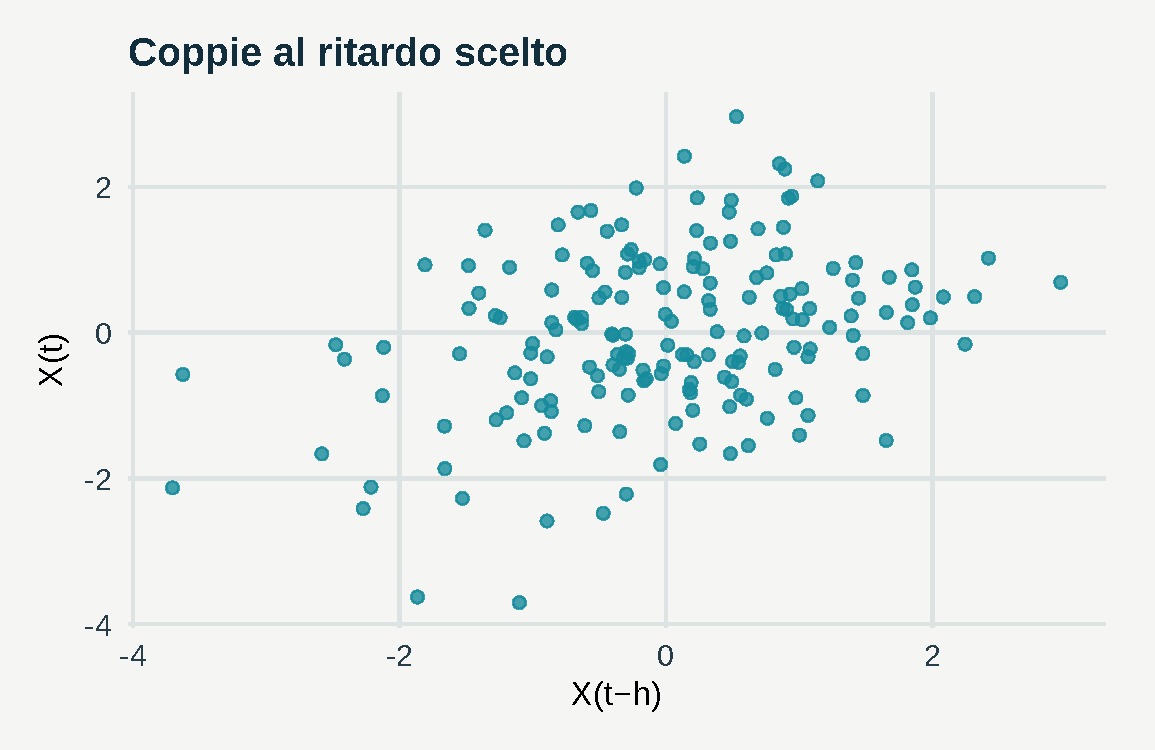
\includegraphics[width=\linewidth,height=5.6cm,keepaspectratio]{Esperimenti/m09-autocorrelazione-B.pdf}\par}
\PSmall{Parametro AR(1): 0,7 $\to$ 0,2. Tutti gli altri parametri e il seme sono fissi.}
}};
\node[anchor=north west,inner sep=0] at([xshift=10.85cm,yshift=-2.12cm]current page.north west){\Colonna{8.16cm}{\PLabel{Confronto fra gli scenari}
{\fontsize{10.2}{12.8}\selectfont\begin{tabular}{@{}>{\raggedright\arraybackslash}p{0.48\linewidth}@{\hspace{.13cm}}>{\raggedright\arraybackslash}p{0.224\linewidth}@{\hspace{.13cm}}>{\raggedright\arraybackslash}p{0.224\linewidth}@{}}\toprule Grandezza & A & B\\[2.3pt]
\midrule 
Correlazione al ritardo & 0,798 & 0,337\\[2.3pt]
Correlazione teorica & 0,7 & 0,2\\[2.3pt]
\bottomrule\end{tabular}\par}
\vspace{.25cm}\PBody{Con parametro 0,2 la correlazione stimata al ritardo uno scende da 0,798 a 0,337, contro valori teorici di 0,7 e 0,2. Nella serie del Nilo i residui hanno autocorrelazione 0,13 al primo ritardo, più vicina allo scenario B.}
}};
\node[anchor=north east,inner sep=0] at([xshift=17.1cm,yshift=-12.04cm]current page.north west){\fontsize{7.7}{9}\selectfont \href{https://marzione00.github.io/Lab_Geo/\#laboratorio/m09-autocorrelazione}{\color{Classical}\bfseries Apri il laboratorio · m09-autocorrelazione}};
\end{tikzpicture}\end{frame}

\begin{frame}[plain]\hypertarget{slide28}{}
\bookmark[level=1,page=28]{Bootstrap a blocchi di una serie dipendente}
\begin{tikzpicture}[remember picture,overlay]
\PilotChrome{Bootstrap a blocchi di una serie dipendente}{LABORATORI DELLA SPEDIZIONE}{28}{Confrontare ricampionamento individuale e ricampionamento di sequenze temporali.}
\node[anchor=north west,inner sep=0] at([xshift=.96cm,yshift=-2.12cm]current page.north west){\Colonna{9.40cm}{{\centering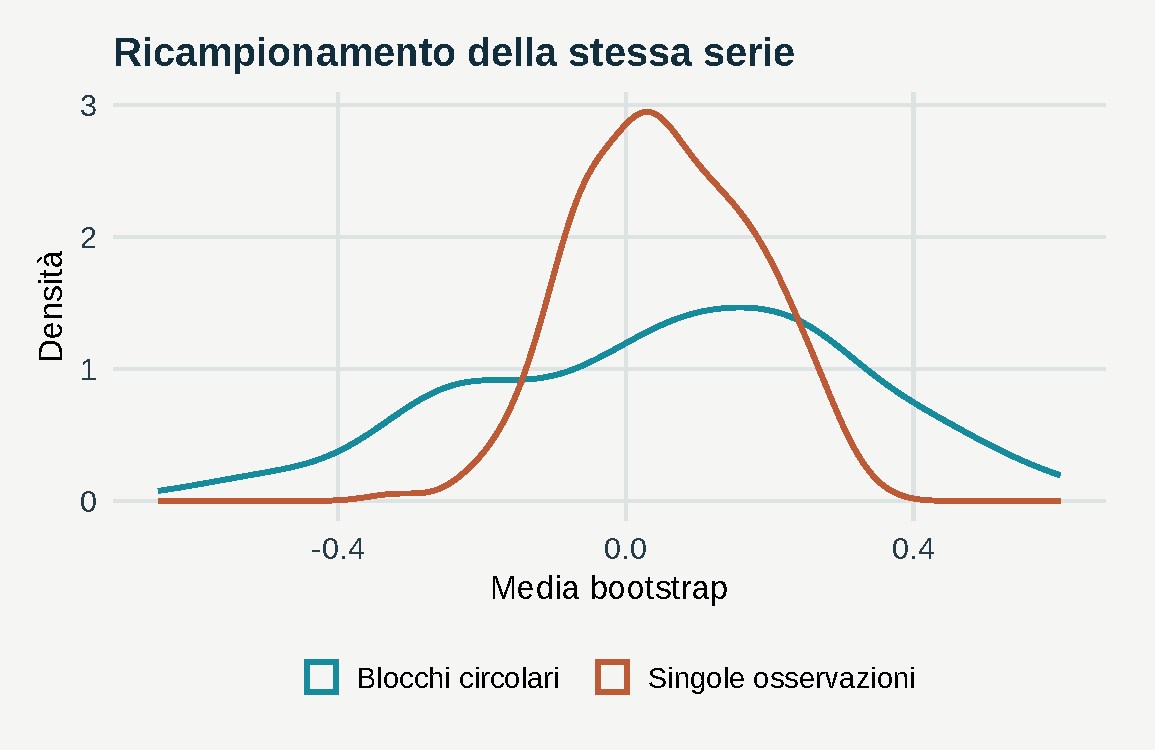
\includegraphics[width=\linewidth,height=6.0cm,keepaspectratio]{Esperimenti/m05-blocchi-A.pdf}\par}
\PSmall{Lunghezza dei blocchi: 8. Seme: 17.}
}};
\node[anchor=north west,inner sep=0] at([xshift=10.85cm,yshift=-2.12cm]current page.north west){\Colonna{8.16cm}{\PLabel{Scenario A · simulazione}
\PBody{La serie sintetica segue un processo AR(1) stazionario. Il ricampionamento individuale estrae valori separatamente, mentre quello a blocchi conserva sequenze di osservazioni consecutive; i blocchi sono circolari, quindi possono proseguire dall’inizio della serie quando raggiungono il termine.}
\par\smallskip{\centering\adjustbox{max width=.98\linewidth}{$\displaystyle B_s=(X_s,\ldots,X_{s+\ell-1}),\quad \bar X^*=n^{-1}\sum_i X_i^*$}\par\smallskip}
\PSmall{$B_s$ è il blocco che inizia all’indice $s$; $\ell$ è la sua lunghezza; $X_i^*$ sono i valori ricampionati; $n$ è la lunghezza della serie ricostruita.}
}};
\node[anchor=north east,inner sep=0] at([xshift=17.1cm,yshift=-12.04cm]current page.north west){\fontsize{7.7}{9}\selectfont \href{https://marzione00.github.io/Lab_Geo/\#laboratorio/m05-blocchi}{\color{Classical}\bfseries Apri il laboratorio · m05-blocchi}};
\end{tikzpicture}\end{frame}

\begin{frame}[plain]\hypertarget{slide29}{}
\bookmark[level=1,page=29]{Confronto | Bootstrap a blocchi di una serie dipendente}
\begin{tikzpicture}[remember picture,overlay]
\PilotChrome{{\fontsize{15.3}{19}\selectfont Confronto | Bootstrap a blocchi di una serie dipendente}}{LABORATORI DELLA SPEDIZIONE}{29}{Il blocco conserva parte della dipendenza locale; la scelta della sua lunghezza contribuisce alla stima dell’incertezza.}
\node[anchor=north west,inner sep=0] at([xshift=.96cm,yshift=-2.12cm]current page.north west){\Colonna{9.40cm}{{\centering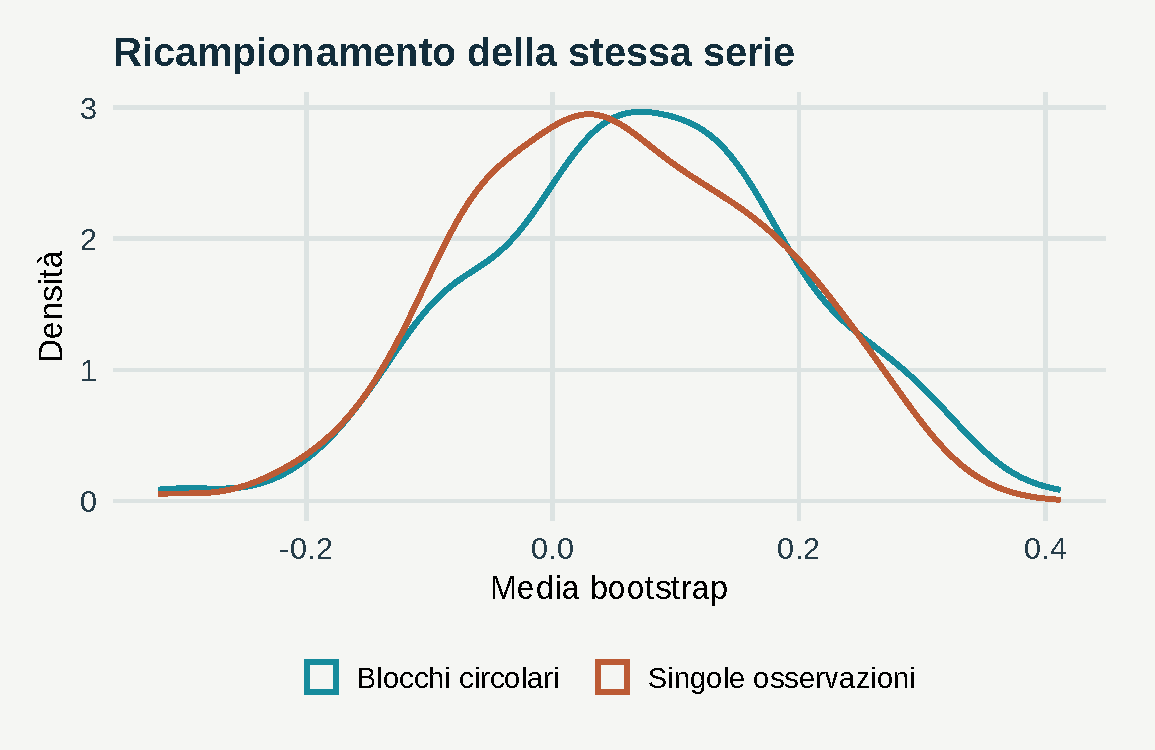
\includegraphics[width=\linewidth,height=5.6cm,keepaspectratio]{Esperimenti/m05-blocchi-B.pdf}\par}
\PSmall{Lunghezza dei blocchi: 8 $\to$ 1. Tutti gli altri parametri e il seme sono fissi.}
}};
\node[anchor=north west,inner sep=0] at([xshift=10.85cm,yshift=-2.12cm]current page.north west){\Colonna{8.16cm}{\PLabel{Confronto fra gli scenari}
{\fontsize{10.2}{12.8}\selectfont\begin{tabular}{@{}>{\raggedright\arraybackslash}p{0.48\linewidth}@{\hspace{.13cm}}>{\raggedright\arraybackslash}p{0.224\linewidth}@{\hspace{.13cm}}>{\raggedright\arraybackslash}p{0.224\linewidth}@{}}\toprule Grandezza & A & B\\[2.3pt]
\midrule 
SE osservazioni & 0,122 & 0,122\\[2.3pt]
SE blocchi & 0,264 & 0,13\\[2.3pt]
Lunghezza del blocco & 8 & 1\\[2.3pt]
Osservazioni originali & 120 & 120\\[2.3pt]
\bottomrule\end{tabular}\par}
\vspace{.25cm}\PBody{Con blocchi di lunghezza uno il bootstrap ricampiona singole osservazioni e il suo errore standard scende da 0,264 a 0,13, vicino a 0,122 della formula per dati indipendenti. Con dipendenza positiva questa riduzione sottostima l’incertezza.}
}};
\node[anchor=north east,inner sep=0] at([xshift=17.1cm,yshift=-12.04cm]current page.north west){\fontsize{7.7}{9}\selectfont \href{https://marzione00.github.io/Lab_Geo/\#laboratorio/m05-blocchi}{\color{Classical}\bfseries Apri il laboratorio · m05-blocchi}};
\end{tikzpicture}\end{frame}

\begin{frame}[plain]\hypertarget{slide30}{}
\bookmark[level=1,page=30]{Dal risultato alla relazione}
\begin{tikzpicture}[remember picture,overlay]
\PilotChrome{Dal risultato alla relazione}{SINTESI}{30}{Riporta differenza, unità, periodi e i due intervalli, dichiarando ritardo massimo e ipotesi asintotiche della covarianza HAC.}
\node[anchor=north west,inner sep=0] at([xshift=.96cm,yshift=-2.12cm]current page.north west){\Colonna{9.40cm}{\PLabel{Domanda di partenza}
\PBody{Di quanto diminuisce il volume annuale del Nilo dopo il 1898, e quanto pesa la dipendenza fra anni?}
\PLabel{Risultato da discutere}
\PBody{La media scende da circa 1097,7 a 853,4 centinaia di milioni di metri cubi, una differenza di −244,3 pari a circa −22,3 per cento. L’intervallo classico va da −302,4 a −186,1; quello HAC con ritardo tre va da −306,4 a −182,1, a stima invariata.}
}};
\node[anchor=north west,inner sep=0] at([xshift=10.85cm,yshift=-2.12cm]current page.north west){\Colonna{8.16cm}{\PLabel{Limiti della conclusione}
\PBody{La soglia del 1898 deriva dalla storia stessa della serie, per cui l’analisi rianalizza un cambiamento già noto. Il contrasto descrive la serie e lascia aperta l’attribuzione a opere idrauliche o a forzanti climatiche, che richiederebbe cronologie e dati del bacino.}
\vspace{.4cm}\href{https://marzione00.github.io/Lab_Geo/\#modulo-P04}{\color{Classical}\bfseries Prosegui · P04 · Un geyser: associazione e previsione}
}};
\end{tikzpicture}\end{frame}

\begin{frame}[plain]\hypertarget{slide31}{}
\bookmark[level=1,page=31]{Fonti, dati e codice per riprodurre le figure}
\begin{tikzpicture}[remember picture,overlay]
\PilotChrome{Fonti, dati e codice per riprodurre le figure}{RIFERIMENTI}{31}{I risultati numerici si riferiscono ai dati e alle ipotesi dichiarate nel caso.}
\node[anchor=north west,inner sep=0] at([xshift=.96cm,yshift=-2.12cm]current page.north west){\Colonna{9.40cm}{\PLabel{Dati e attribuzioni}
\PBody{Serie Nile del pacchetto datasets di R, dalla raccolta di Cobb (1978): volumi annuali del Nilo ad Aswan, 1871-1970. La covarianza HAC segue la formulazione di Newey e West con pesi di Bartlett, confrontata con cov\_hac di statsmodels.}
}};
\node[anchor=north west,inner sep=0] at([xshift=10.85cm,yshift=-2.12cm]current page.north west){\Colonna{8.16cm}{\PLabel{Nell’archivio dei sorgenti}
\PBody{Codice contiene i frammenti delle pagine; R contiene lo script P03\_figure.R, che ricostruisce figure e valori dai dati. Esperimenti comprende i programmi dei due scenari, Diagrammi i disegni TikZ modificabili, Scena il modello Blender della copertina.}
\vspace{.4cm}\href{https://marzione00.github.io/Lab_Geo/\#modulo-P03}{\color{Classical}\bfseries Apri la spedizione P03 su GeoStat Lab}
}};
\end{tikzpicture}\end{frame}
\end{document}
